\documentclass[11pt,a4paper]{article}
\usepackage{estilosexercicios}
\usepackage{hyperref}

%\usepackage[bottom=2cm,top=3cm,left=3cm,right=2cm]{geometry}
%\usepackage[utf8]{inputenc}
%Environments para esta lista
% ---------------------------------------------------
\definecolor{Floresta}{rgb}{0.13,0.54,0.13}
\newcommand{\exercicio}[1]{\subsection{Exercício #1} \textcolor{blue}{\bf(#1)}}
\newcommand{\dividiritens}[1]{\begin{tasks}[counter-format={(tsk[a])},label-width=3.6ex, label-format = {\bfseries}, column-sep = {0pt}](1) #1 \end{tasks}}

\newcommand{\dividiritensdiv}[2]{\begin{tasks}[counter-format={(tsk[a])},label-width=3.6ex, label-format = {\bfseries}, column-sep = {0pt}](#1) #2 \end{tasks}}

\newcommand{\pers}[1]{\textcolor{Floresta}{$\negrito{(#1)} $}}

\newcommand{\solucao}[1]{
\textbf{\\ \\ \textcolor{red}{Solução:}} #1}
\newcommand{\figura}[1]{\input Arquivos_de_figs_Exercicios/#1} %Adicionar figuras do latex

\newcommand{\m}[2]{\mathcal{M}_{#1}(#2)} %Desculpe, cansei de escrever isso toda hora 

% ---------------------------------------------------
\title{Álgebra Linear}
\author{MAT5730}
\date{2° semestre de 2019}

\begin{document}
\definecolor{Floresta}{rgb}{0.13,0.54,0.13}
\maketitle
\tableofcontents
\newpage
\begin{comment}

\begin{center}
\large\textbf{\textcolor{Floresta}{Lista 1}}\\
\end{center}

\end{comment}

\section{\textcolor{Floresta}{Lista 0}}


\exercicio{1}


\newpage
\section{\textcolor{Floresta}{Lista 1}}


\exercicio{1} Sejam $V$ um $K$-espaço vetorial e $W$ um subespaço de $V.$ Seja $S = \{v_i\}_{i\in I} \subset V$ tal que $\overline{S} = \{v_i + W\}_{i\in I}$ é linearmente independente no espaço quociente $V/W.$ Mostre que se $A$ é um conjunto linearmente independente de $W$ então $S \cup A$ é um conjunto linearmente independente de $V.$
\solucao{Se $\overline{S} = \{\overline{v_i} = v_i + W\}_{i\in I}$ é LI em $V/W,$ isso significa que, para todo $M \subseteq I$ finito, temos que, para $\alpha_m \in K,$ com $m \in M,$ ocorre
\[
\sum\limits_{m \in M} \alpha_m \overline{v_m} = 0 \Rightarrow \alpha_m = 0 \ \forall \ m \in M
\]

Seja $A = \{ w_j \}_{j \in J}.$ Por hipótese, sabemos também que $A$ é um conjunto linearmente independente, ou seja, para todo $N \subseteq I$ finito, temos que, para $\alpha_n \in K,$ com $n \in N,$ ocorre
\[
\sum\limits_{n \in N} \alpha_n w_n = 0 \Rightarrow \alpha_n = 0, \ \forall \ n \in N
\]

Para mostrar que $S \cup A = \{v_i\}_{i\in I} \cup \{ w_j \}_{j \in J} = \{ u_p \}_{p \in I \cup J}$ é um conjunto linearmente independente de $V,$ precisamos mostrar que, para todo $L \subset I \cup J$ finito, temos que, para $\alpha_\ell \in L,$ com $\ell \in L,$ ocorre
\[
\sum\limits_{\ell \in L} \alpha_\ell u_\ell = 0 \Rightarrow \alpha_\ell = 0, \ \forall \ \ell \in L
\]

Para fazer isso, precisamos antes verificar se existem vetores que são comuns aos dois subconjuntos, ou seja, calcular $S \cap A.$ Observe que
\[
s \in S \Rightarrow \overline{s} \in \overline{S} 
\]
Como $\overline{S}$ é um conjunto linearmente independente em $W,$ temos que $\overline{s} \neq \overline{0}.$ Portanto, segue que $s - 0 \notin W \Rightarrow s \notin W.$
Mas como $A \subseteq W,$ então isso quer dizer que $s \notin A.$ Portanto, concluímos que $S \cap A = \emptyset.$ Isso quer dizer que todos os $v_i$'s são diferentes dos $w_j$'s, e mais ainda, que $I \cup J$ é uma união disjunta.

Logo, considerando novamente $S \cup A = \{v_i\}_{i\in I} \cup \{ w_j \}_{j \in J}$, para todo $L \subseteq I \cup J$ finito, existem $I^{\prime} \subseteq I$ e $J^{\prime} \subseteq J$ tais que $I^{\prime} \cup J^{\prime} = L.$ Desse modo, temos que
\[
\sum\limits_{\ell \in L} \alpha_\ell u_\ell = 0 \Rightarrow
\]
\[
\sum\limits_{i \in I^{\prime}} \alpha_i v_i + \sum\limits_{j \in J^{\prime}} \alpha_j w_j = 0 \quad \mbox{em } V \Rightarrow 
\]\[
\overline{\sum\limits_{i \in I^{\prime}} \alpha_i v_i + \sum\limits_{j \in J^{\prime}} \alpha_j w_j} = \overline{0} \quad \mbox{em } V/W \Rightarrow 
\]
\[
\sum\limits_{i \in I^{\prime}} \alpha_i \overline{v_i} + \underbrace{\sum\limits_{j \in J^{\prime}} \alpha_j \overline{w_j}}_{= 0, \mbox{ pois } w_j \in W}  = \overline{0} \Rightarrow \sum\limits_{i \in I^{\prime}} \alpha_i \overline{v_i} = \overline{0} \Rightarrow \alpha_i = 0 \ \forall \ i \in I^{\prime},
\]
pois $\{v_i\}_{i \in I^{\prime}} \subseteq \overline{S}$ é um conjunto linearmente independente.

Assim, usando agora o fato de que $\{w_j\}_{j \in J^{\prime}} \subseteq A$ é um conjunto linearmente independente em $W,$ temos que
\[
\textcolor{red}{\sum\limits_{i \in I^{\prime}} \alpha_i v_i} + \sum\limits_{j \in J^{\prime}} \alpha_j w_j = 0 \Rightarrow \textcolor{red}{0} + \sum\limits_{j \in J^{\prime}} \alpha_j w_j = 0 \Rightarrow  \sum\limits_{j \in J^{\prime}} \alpha_j w_j = 0 \Rightarrow \alpha_j = 0 \ \forall \ j \in  J^{\prime}
\]
Concluímos portanto que
\[
\sum\limits_{\ell \in L} \alpha_\ell u_\ell = 0 \Rightarrow \alpha_\ell = 0 \ \forall \ \ell \in L
\]
Daí, $S \cup A$ é um conjunto linearmente independente em $V.$
}

\exercicio{2} Sejam $V$ um $K$-espaço vetorial e $W$ um subespaço de $V.$ Seja $S = \{v_i\}_{i \in I} \subset V$ tal que $S = \{v_i + W\}_{i \in I}$ gera o espaço quociente $V/W.$ Mostre que se $A$ é um conjunto gerador de
$W$ então $S \cup A$ é um conjunto gerador de $V$.
\solucao{
Se $\overline{S} = \{\overline{v_i} = v_i + W\}_{i\in I}$ gera em $V/W,$ isso significa que, para todo $\overline{v} \in V/W,$ existem $M \subseteq I$ finito e $\alpha_m \in K,$ com $m \in M,$ tais que
\[
\overline{v} = \sum\limits_{m \in M} \alpha_m \overline{v_m}
\]

Seja $A = \{ w_j \}_{j \in J}.$ Por hipótese, sabemos também que $A$ gera $W$, ou seja, para todo $w \in W,$ existem $N \subseteq J$ finito e $\alpha_n \in K,$ com $n \in N,$ tais que
\[
w = \sum\limits_{n \in N} \alpha_n w_n
\]

Precisamos mostrar que $S \cup A = \{v_i\}_{i\in I} \cup \{ w_j \}_{j \in J} = \{ u_p \}_{p \in I \cup J}$ é um conjunto gerador para $V,$ ou seja, que para todo $v \in V,$ existem $L \subset I \cup J$ finito e $\alpha_\ell \in K,$ com $\ell \in L,$ tais que
\[
v = \sum\limits_{\ell \in L} \alpha_\ell u_\ell
\]
Note que, como $\overline{S}$ é um conjunto gerador de $V/W,$ temos como já foi explicitado acima que, para $\overline{v} \in V/W,$
\[
\overline{v} = \sum\limits_{m \in M} \alpha_m \overline{v_m} \Rightarrow \overline{v} - \sum\limits_{m \in M} \alpha_m \overline{v_m} = \overline{0} \Rightarrow v - \sum\limits_{m \in M} \alpha_m v_m \in W
\]
Como $A = \{ w_j \}_{j \in J}$ é conjunto gerador para $W,$ temos que existem $N \subseteq J$ finito e $\alpha_n \in K,$ com $n \in N,$ tais que
\[
v - \sum\limits_{m \in M} \alpha_m v_m  = \sum\limits_{n \in N} \alpha_n w_n
\]
Assim, tomando $L = N \cup M$:
\[
v  = \sum\limits_{m \in M} \alpha_m v_m + \sum\limits_{n \in N} \alpha_n w_n \Rightarrow v = \sum\limits_{\ell \in L} \alpha_\ell u_\ell
\]
Portanto, $S \cup A$ é um conjunto gerador para $V.$
}

\exercicio{3} Seja $V$ um $K$-espaço vetorial e sejam $U$ e $W$ subespaços de $V.$ Prove:
\dividiritens{
    \task[\pers{a}] O Segundo Teorema do Isomorfismo:
    \[
    \frac{U + W}{W} \cong \frac{U}{U \cap W}.
    \]
        \task[\pers{b}] O Terceiro Teorema do Isomorfismo: Se $U \subset W,$
        \[
        \frac{V}{W} \cong \frac{V/U}{W/U}
        \]
}

\solucao{}

\exercicio{4} Seja $V$ um $K$-espaço vetorial e sejam $U$ e $W$ subespaços de $V$ tais que $\dim (V/U) = m$ e $\dim (V/W) = n.$ Prove que $\dim (V/(U \cap W)) \le m + n.$

\solucao{Das informações fornecidas no enunciado, sabemos que:
\[
\dim (V/U) = m \Rightarrow \dim(V) - \dim(U) = m
\]
\[
\dim (V/W) = n \Rightarrow \dim(V) - \dim(W) = n
\]
Somando essas duas equações obtemos:
\[
2\dim(V) - (m+n) = \dim(U) + \dim(W).
\]
Sabemos também que, se $U$ e $W$ são subespaços de $V,$ então
\[
\dim(U) + \dim(W) = \dim(U \cap W) + \dim(U + W)
\]

Estamos interessados em encontrar $\dim(V/(U \cap W)) = \dim(V) - \dim(U \cap W).$
Observe que, como $U$ e $W$ são subespaços de $V,$ então $\dim(V) \ge \dim(U + W).$ Desse modo,
\[
\dim(U) + \dim(W)  = \dim(U \cap W) + \textcolor{Blue}{\dim(U + W)} \le \dim(U \cap W) + \textcolor{Blue}{\dim(V)} 
\]
Então:
\[
\textcolor{Verde}{\dim(U) + \dim(W)} \le \dim(U \cap W) +\dim(V) \Rightarrow \textcolor{Verde}{2\dim(V) - (m+n) } \le \dim(U \cap W) +\dim(V) \Rightarrow \]\[-(m+n) \le \dim(U \cap W) - \dim(V) \Rightarrow \dim(V) -  \dim(U \cap W) \le m+n
\]
Portanto, concluímos que
\[
\dim(V/(U \cap W)) = dim(V) -  \dim(U \cap W) \le m+n \Rightarrow \boxed{\dim(V/(U \cap W))  \le m + n}
\]
}

\exercicio{5} Mostre que
\dividiritens{
    \task[\pers{a}] $W \oplus U= W^{\prime} \oplus U^{\prime} \ \mbox{e} \ W \cong W^{\prime} \nrightarrow U \cong U^{\prime}.$
   \task[\pers{b}] $V \cong V^{\prime}, V = W \oplus U \ \mbox{e} \ V^{\prime} = W \oplus U^{\prime} \nrightarrow U \cong U^{\prime}.$
}


\solucao{
\dividiritens{
    \task[\pers{a}] Considere $K$ um corpo, e seja
    \[
    V = \bigoplus_{i=1}^\infty Ke_i
    \]
Considere 
\[
    W = \bigoplus_{i=1}^\infty Ke_{2i}
\]
Observe que $W \subseteq V,$ e além disso, $W \cong V.$ Temos também que 
\[
V = W \oplus \left(  \bigoplus_{i=1}^\infty Ke_{2i+1} \right)
\]
Portanto, tomando
\[
W = \bigoplus_{i=1}^\infty Ke_{2i}, \ U = \bigoplus_{i=1}^\infty Ke_{2i+1}, \ W^{\prime} = V, \ \mbox{e} \ U^{\prime} = \{ 0 \},
\]
temos que
\[
\left( \bigoplus_{i=1}^\infty Ke_{2i} \right) \oplus \left(  \bigoplus_{i=1}^\infty Ke_{2i+1} \right) \cong V \cong V \oplus \{ 0 \} \Rightarrow W \oplus U= W^{\prime} \oplus U^{\prime}
\]
e
\[
\bigoplus_{i=1}^\infty Ke_{2i} \cong \bigoplus_{i=1}^\infty Ke_i \Rightarrow W \cong W \prime,
\]
mas
\[
\bigoplus_{i=1}^\infty Ke_{2i+1} \ncong \{ 0 \} \Rightarrow U \ncong U^{\prime}
\]
        \task[\pers{b}] 
    }
\textbf{Observação:} Cabe salientar que ambos os itens dessa questão são válidos quando $V$ é um espaço vetorial de dimensão finita.
}

\exercicio{6} Seja $V$ um espaço vetorial e seja $W$ um subespaço de $V.$ Suponha que $V = V_1 \oplus \ldots \oplus V_n$ e $S = S_1 \oplus \ldots \oplus S_n,$ com $S_i \subseteq V_i$ subespaços de $V$ para todo $i = 1, \ldots, n.$ Mostre que
\[
\frac{V}{S} \cong \frac{V_1}{S_1} \oplus \ldots \oplus \frac{V_n}{S_n}.
\]
\solucao{
Sabemos que, se $V$ é soma direta de $ V_1 \oplus \ldots \oplus V_n,$ então todo $v \in V$ pode ser escrito como soma de elementos de $V_i$ \textbf{de maneira única}. Podemos escrever então
\[v = \sum\limits_{i = 1}^n v_i\]

O mesmo se aplica a $S.$ Dito isso, considere a aplicação
\[
\fullfunction{T}{V = \bigoplus\limits_{i=1}^n V_i = V_1 \oplus \ldots \oplus V_n}{\bigoplus\limits_{i=1}^n  \frac{V_i}{S_i} =  \frac{V_1}{S_1} \oplus \ldots \oplus \frac{V_n}{S_n} }{v = \sum\limits_{i = 1}^n v_i}{T(v) = \sum\limits_{i = 1}^n (v_i + S_i)}
\]
Verifiquemos que $T$ é uma transformação linear:
\begin{itemize}
    \item Para todo $u, v \in V,$ podemos escrever de maneira única $u = \sum\limits_{i =1}^n u_i$ e $v = \sum\limits_{i =1}^n v_i$. Portanto, temos
    \[T(u) + T(v) = T\left(\sum\limits_{i=1}^n u_i \right) + T\left(\sum\limits_{i=1}^n v_i \right) = \sum\limits_{i=1}^n (u_i + S_i) +  \sum\limits_{i=1}^n (v_i + S_i) =  \]\[\sum\limits_{i=1}^n ((u_i + S_i) + (v_i + S_i)) = T(u + v) \Rightarrow T(u) + T(v) = T(u+v).\]
    \item Para todo $v \in V,$ podemos escrever de maneira única $v = \sum\limits_{i =1}^n v_i;$ assim, para $\alpha \in K:$
    \[
    T(\alpha v) = T\left(\alpha \sum\limits_{i=1}^n v_i \right) =   T\left( \sum\limits_{i=1}^n \alpha v_i \right) = T\left( \sum\limits_{i=1}^n \alpha v_i \right) = \sum\limits_{i=1}^n (\alpha v_i + S_i) = \]\[ \sum\limits_{i=1}^n \alpha (v_i + S_i)  = \alpha \sum\limits_{i=1}^n (v_i + S_i) = \alpha T(v) \Rightarrow T(\alpha v) = \alpha T(v) 
    \]
\end{itemize}
Logo, $T$ é uma transformação linear. Vamos utilizar o Primeiro Teorema do Isomorfismo em $T.$ Para isso, calculemos o núcleo e a imagem de $T:$
\begin{itemize}
    \item $\mbox{Im} (T):$ Dado $u \in \bigoplus\limits_{i=1}^n  \frac{V_i}{S_i},$ temos que esse elemento pode ser escrito de maneira única como 
    \[
    u = \sum\limits_{i = 1}^n (u_i + S_i),
    \]
    onde $u_i \in V_i.$ Então temos que
        \[
    u = \sum\limits_{i = 1}^n (u_i + S_i) = T\left(  \sum\limits_{i = 1}^n u_i \right).
    \]
    Logo, $T$ é sobrejetora, e 
    \[
    \mbox{Im}(T) = \bigoplus\limits_{i=1}^n  \frac{V_i}{S_i} =  \frac{V_1}{S_1} \oplus \ldots \oplus \frac{V_n}{S_n} 
    \]
    \item $\mbox{Ker} (T):$ Considere $v \in \mbox{Ker}(T).$ Então, tomando $v = \sum\limits_{i=1}^n v_i,$ temos que
    \[
 v \in \mbox{Ker}(T) \Rightarrow T(v) = 0 \Rightarrow T\left(\sum\limits_{i=1}^n v_i \right) = 0 \Rightarrow \sum\limits_{i=1}^n (v_i + S_i) = 0 \Rightarrow \]\[v_i + S_i = 0, \ \forall i \in  \{1, \ldots, n\} \Rightarrow v_i \in S_i , \ \forall i \in  \{1, \ldots, n\} \Rightarrow v \in S
    \]
    Assim, $\mbox{Ker}(T) \subseteq S.$
    Agora, tome $s \in S.$ Então, como $S = \bigoplus\limits_{i=1}^n S_i,$ então podemos escrever $s$ de maneira única como
    \[
    s = \sum\limits_{i = 1}^n s_i,
    \]
    onde $s_i \in S_i,$ para $i = 1, \dots, n.$
    Desse modo,
    \[
    T(s) = T\left(  \sum\limits_{i = 1}^n s_i \right) = \sum\limits_{i = 1}^n (s_i + S_i) = \underbrace{\sum\limits_{i = 1}^n (0 + S_i)}_{\mbox{pois } s_i \in S_i \ \forall i} = 0.
    \]
    Assim, $S \subseteq \mbox{Ker}(T).$
    Concluímos que $\mbox{Ker}(T) = S.$
\end{itemize}

Pelo Primeiro Teorema do Isomorfismo, temos que
\[
    \frac{V}{\textcolor{Blue}{\mbox{Ker}(T)}} \cong \textcolor{Verde}{\mbox{Im}(T)} \Rightarrow  \frac{V}{\textcolor{Blue}{S}} \cong \textcolor{Verde}{ \bigoplus\limits_{i=1}^n  \frac{V_i}{S_i}} 
\]
Então:
\[
\frac{V}{S} \cong \frac{V_1}{S_1} \oplus \ldots \oplus \frac{V_n}{S_n},
\]
como queríamos.
}

\exercicio{7} Seja $V$ um $K$-espaço vetorial e seja $W$ um subespaço de $V.$ Seja $T \in \mathcal{L}(V)$ e defina $\overline{T} \colon V/W \to V/W$ por
\[
\overline{T}(v+ W) = T(v) + W, \mbox{ para todo } v + W \in V/W.
\]
\dividiritens{
    \task[\pers{a}]  Determine uma condição necessária e suficiente sobre $W$ para que $\overline{T}$ esteja bem definida.
   \task[\pers{b}]  Se $\overline{T}$ estiver bem definida, mostre que ela é linear e determine seu núcleo e sua imagem.
}
\solucao{
\dividiritens{
    \task[\pers{a}] Seja
    \[   \fullfunction{\pi}{V}{V/W}{v}{\pi(v) = v +W}\]
    A projeção canônica de $V$ em $V/W.$ Então, podemos considerar o seguinte diagrama:
    

\begin{center}

\tikzset{every picture/.style={line width=0.75pt}} %set default line width to 0.75pt        

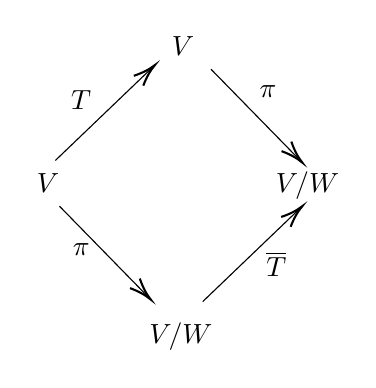
\begin{tikzpicture}[x=0.75pt,y=0.75pt,yscale=-1,xscale=1]
%uncomment if require: \path (0,300); %set diagram left start at 0, and has height of 300

%Straight Lines [id:da34889049551168805] 
\draw    (62.5,94) -- (109.06,49.38) ;
\draw [shift={(110.5,48)}, rotate = 496.22] [color={rgb, 255:red, 0; green, 0; blue, 0 }  ][line width=0.75]    (10.93,-3.29) .. controls (6.95,-1.4) and (3.31,-0.3) .. (0,0) .. controls (3.31,0.3) and (6.95,1.4) .. (10.93,3.29)   ;

%Straight Lines [id:da3558445685185325] 
\draw    (133.5,162) -- (180.06,117.38) ;
\draw [shift={(181.5,116)}, rotate = 496.22] [color={rgb, 255:red, 0; green, 0; blue, 0 }  ][line width=0.75]    (10.93,-3.29) .. controls (6.95,-1.4) and (3.31,-0.3) .. (0,0) .. controls (3.31,0.3) and (6.95,1.4) .. (10.93,3.29)   ;

%Straight Lines [id:da04986735852274893] 
\draw    (137.5,50) -- (180.1,93.57) ;
\draw [shift={(181.5,95)}, rotate = 225.64] [color={rgb, 255:red, 0; green, 0; blue, 0 }  ][line width=0.75]    (10.93,-3.29) .. controls (6.95,-1.4) and (3.31,-0.3) .. (0,0) .. controls (3.31,0.3) and (6.95,1.4) .. (10.93,3.29)   ;

%Straight Lines [id:da9800428074288963] 
\draw    (64.5,116) -- (107.1,159.57) ;
\draw [shift={(108.5,161)}, rotate = 225.64] [color={rgb, 255:red, 0; green, 0; blue, 0 }  ][line width=0.75]    (10.93,-3.29) .. controls (6.95,-1.4) and (3.31,-0.3) .. (0,0) .. controls (3.31,0.3) and (6.95,1.4) .. (10.93,3.29)   ;


% Text Node
\draw (124,39) node  [align=left] {$V$};
% Text Node
\draw (59,105) node  [align=left] {$V$};
% Text Node
\draw (184,106) node  [align=left] {$V/W$};
% Text Node
\draw (123,179) node  [align=left] {$V/W$};
% Text Node
\draw (75,65) node  [align=left] {$T$};
% Text Node
\draw (165,61) node  [align=left] {$\displaystyle \pi $};
% Text Node
\draw (75,137) node  [align=left] {$\displaystyle \pi $};
% Text Node
\draw (169,144) node  [align=left] {$\displaystyle \overline{T}$};


\end{tikzpicture}

\end{center}
Note que $\pi \circ T = \overline{T} \circ \pi.$ Daí, $\overline{T}$ estará bem-definida se $\Ker(\pi) \subseteq \Ker(\pi \circ T).$ Claramente, temos que $\Ker(\pi) = W.$ Vamos calcular $ \Ker(\pi \circ T).$ Temos que
\[v \in \Ker(\pi \circ T) \Leftrightarrow  \pi ( T(v)) = \overline{0} \Leftrightarrow T(v) \in W \Leftrightarrow v \in T^{-1}\]

Logo, temos que 
\[\textcolor{Blue}{\Ker(\pi)} \subseteq \textcolor{Verde}{\Ker(\pi \circ T)} \Rightarrow \textcolor{Blue}{W} \subseteq \textcolor{Verde}{T^{-1}(W)} \Rightarrow T[W] \subseteq W.\]
Portanto, uma condição necessária e suficiente para $\overline{T}$ estar bem definida é que para todo $v \in W,$ tenhamos $T(v) \in W,$ ou seja, $T(W) \subseteq W.$

Em outras palavras, $\overline{T}$ está bem definida se $W$ for um subespaço $T$-invariante de $V.$
    \task[\pers{b}] Verifiquemos que $\overline{T}$ é uma transformação linear. Temos:
    \begin{itemize}
        \item[$\textcolor{red}{\vardiamond}$] Para todos $u + W, v + W \in V/W,$ lembrando que $T$ é linear, temos que
     \[        \overline{T}((u+W) + (v + W)) = \overline{T}((u+v)+ W) = \textcolor{RawSienna}{T(u+v)} + W = \textcolor{RawSienna}{T(u)+T(v)}+ W = \]\[\textcolor{red}{(T(u) + W)} + \textcolor{Laranja}{(T(v) + W)} = \textcolor{red}{\overline{T}(u+W)} + \textcolor{Laranja}{\overline{T}(v+W)}      \]
        Logo, $\overline{T}(\overline{u}+\overline{v}) = \overline{T}(\overline{u})+ \overline{T}(\overline{v}).$
        
       \item[$\clubsuit$] Para todo $v + W \in V/W,$ e para todo $\alpha \in K,$ temos que
       \[         \overline{T}(\alpha(v+W)) = \overline{T}( (\alpha v)+W) = \textcolor{RawSienna}{T(\alpha v)} + W = \textcolor{RawSienna}{\alpha T(v)} + W =  \]\[ \alpha \textcolor{Laranja}{(T(v) +W)} = \alpha \textcolor{Laranja}{\overline{T}(v + W)}       \]
        Portanto, $\overline{T}(\alpha \overline{v}) = \alpha \overline{T}(\overline{v}).$
    \end{itemize}
    
    Vamos encontrar o núcleo e a imagem de $\overline{T}.$
    \begin{itemize}
        \item[$\textcolor{red}{\varheart}$] Sendo $\overline{v} = v + W \in V/W,$ observe que
        \[
        \overline{T}(\overline{v}) = 0 \Rightarrow \overline{T(v)}=0 \Rightarrow T(v) \in W \Rightarrow v \in T^{-1}(W).
        \]
        Portanto, temos que
        \[
        \Ker(\overline{T}) = \{ \overline{v} | v \in T^{-1}(W) \}.
        \]
        
     \item[$\spadesuit$] Vamos verificar que $\overline{T}$ é sobrejetora. Sabemos que $\pi$ é sobrejetora. Então, temos que
     \[
     \begin{array}{lcr}
     \mbox{Im}(\overline{T}) &=&    \mbox{Im}(\overline{T} \circ \pi) \\
     &=&    \mbox{Im}(\pi \circ T) \\
     &=&    \{ \pi(T(v)) : v \in V \} \\
     &=&    \{ \overline{T(v)} : v \in V \} \\
     \end{array}
     \]
     Portanto, temos que
     \[
     \mbox{Im}(\overline{T}) = V/W.
     \]
    \end{itemize}

}
    }

\exercicio{8} Seja $T \in \mathcal{L}(\mathbb{R}^3)$ o operador linear definido por $T(x, y, z) = (x, x, x).$ Seja $T \colon \mathbb{R}^3/W \to \mathbb{R}^3/W$
tal que $\overline{T}((x, y, z) + W) = T(x, y, z) + W,$ em que $W = \mbox{Ker } T.$ Descreva $\overline{T}.$

\solucao{Veja que $\overline{T}$ está bem definida, pois $W = \Ker (T)$ é um subespaço $T$-invariante de $V.$ Vamos encontrar o núcleo e a imagem de $\overline{T}.$
\begin{itemize}
    \item Do exercício anterior, temos que
            \[
        \Ker(\overline{T}) = \{ \overline{v} | v \in T^{-1}(W) \}.
        \]
        Em particular,
                    \[  \Ker(\overline{T}) = \{ \overline{v} | v \in T^{-1}(\Ker T) \} = \{ \overline{v} | v \in T^{-1}(\Ker T) \} \]
        Então segue que
        \[
        v \in T^{-1}(\Ker T)  \Rightarrow T(v) \in \Ker(T) \Leftrightarrow T(T(v)) = 0.
        \]
        Mas $T(T(v)) = T(v).$ De fato, para $v = (x,y,z) \in \mathbb{R}^3,$ temos 
        \[
        T(T(v)) = T(\textcolor{Cyan}{T(x,y,z)}) = T(\textcolor{Cyan}{x,x,x}) = (x,x,x) = T(x,y,z) = T(v)
        \]
        Daí, como para $v \in T^{-1}(\Ker T),$ temos $T(T(v)) = 0,$
        \[
        \textcolor{Emerald}{T(T(v))} = 0 \Rightarrow  \textcolor{Emerald}{T(v)} = 0
        \]
        
    Além disso, se $v \in \Ker (T) = W,$ temos $\overline{v} = 0.$
    
    Portanto, concluímos que $\Ker (\overline{T}) = \{ 0 \},$ ou seja, $\overline{T}$ é injetora.
    \item Do exercício anterior, temos
       \[
     \mbox{Im}(\overline{T}) = V/W.
     \]
     Logo, $\mbox{Im}(\overline{T}) = \mathbb{R}^3/\Ker T.$
     Podemos também descrever $\mbox{Im}(\overline{T})$ da seguinte maneira:
     \[
     \begin{array}{rcl}
     \mbox{Im}(\overline{T}) &=& \{ \overline{T(v)} : v \in V \} \\
     &=& \{ T(v) + \Ker T | v = (x,y,z) \in \mathbb{R}^3 \} \\
     &=& \{ (x,x,x) +  \textcolor{PineGreen}{\Ker T} | x \in \mathbb{R} \} \\
     &=& \{ (x, x,x) + \textcolor{PineGreen}{(0,y,z)} | x,y,z \in \mathbb{R} \} \\
        &=& \{ (x, x+y,x+z) | x,y,z \in \mathbb{R} \} \\  
     \end{array}
     \]
\end{itemize}

}

\exercicio{9} Sejam $V$ e $U$ $K$-espaços vetoriais. Seja $W$ um subespaço de $V$ e $\pi \colon V \to V/W$ a projeção canônica. Mostre que a função $\mathcal{L}(V/W, U) \to \mathcal{L}(V, U),$ dada por $T \to T \circ \pi,$ é injetora.

\solucao{
Temos a função\[\fullfunction{\varphi}{\mathcal{L}(V/W, U)}{ \mathcal{L}(V, U)}{T}{T \circ \pi}\]Para mostrar que $\varphi$ é injetora, precisamos verificar que, para $T \in \mathcal{L}(V/W, U),$ se $\varphi(T) = 0,$ então $T \cong 0.$ Note que
\[
\varphi(T) = 0 \Rightarrow T \circ \pi = 0 \Rightarrow T(\pi(v)) = 0.
\]
Vamos mostrar que $T(u) = 0 \ \forall u \in V/W.$ Sabemos que $\pi$ é sobrejetora. Assim, dado $u \in V/W,$ existe $v \in V$ tal que $u = \pi(v).$ Logo,
\[
T(\textcolor{Green}{u}) = T(\textcolor{Green}{ \pi(v)}) = (T \circ \pi)(v) = 0.
\]
Portanto, $T(u) = 0 \ \forall u \in V/W.$ Daí, $\Ker (\varphi) = \{ 0 \}.$

Concluímos que $\varphi$ é injetora.

%Verifiquemos primeiramente que $\varphi$ é uma transformação linear:\[(\varphi(S) - \varphi(T))(v) = \varphi(S - T)(v) = ((S - T) \circ \pi)(v) = (S-T)(\pi(v)) = S\]
}

\exercicio{10} Seja $V$ um $K$-espaço vetorial e seja $W$ um subespaço de $V.$ Mostre que $(V/W)^{*} \cong W^{0}$ e que $V^{*}/W^{0} \cong W^{*}.$

\solucao{Mostremos que $(V/W)^{*} \cong W^{0}.$ Para isso, a ideia será utilizar a aplicação canônica de $V$ em $V/W$ e sua transposta, e depois aplicar o Primeiro Teorema do Isomorfismo para obter o resultado desejado. Comecemos considerando a aplicação canônica
\[
\fullfunction{T}{V}{V/W}{v}{T(v) = v + W}
\]
Veja que $T$ é sobrejetora (isto é, $\mbox{Im } T = V/W$), e $\mbox{Ker } T = W.$ Consideremos a aplicação transposta
\[\fullfunction{T^t}{(V/W)^{*}}{V^{*}}{f}{T^t(f) = f \circ T}
\]
Das propriedades da transformação transposta, sabemos que
\[
\mbox{Ker } T^t = (\textcolor{Laranja}{\mbox{Im } T})^{0} = (\textcolor{Laranja}{V/W})^{0} = \{0\}
\]
\[
\mbox{Im } T^t = (\textcolor{Rosadif}{\mbox{Ker } T})^{0} = \textcolor{Rosadif}{W}^{0}
\]
Pelo Primeiro Teorema do Isomorfismo, temos que
\[
\frac{(V/W)^{*}}{\textcolor{Laranja}{\mbox{Ker } T^t}} \cong \textcolor{Rosadif}{\mbox{Im } T^t } \Rightarrow \frac{(V/W)^{*}}{\textcolor{Laranja}{\{ 0 \}}} \cong \textcolor{Rosadif}{W^{0}} \Rightarrow \boxed{ (V/W)^{*} \cong W^0}
\]

Mostremos agora que $V^{*}/W^{0} \cong W^{*}.$ Utilizaremos a mesma estratégia, mas considerando agora a inclusão. Tome a inclusão de $W$ em $V,$ isto é:
\[
\fullfunction{\iota}{W}{V}{w}{\iota(w) = w}
\]
Note que $\mbox{Ker }\iota = \{ 0 \}$ e $\mbox{Im } \iota = W.$
Seja
\[
\fullfunction{\iota^t}{V^{*}}{W^{*}}{f}{\iota(f) = f \circ \iota}
\]
a transposta de $\iota.$ Observe que
\[
\mbox{Ker } \iota^t = (\textcolor{Laranja}{\mbox{Im } \iota})^{0} = \textcolor{Laranja}{W}^{0} 
\]
\[
\mbox{Im } \iota^t = (\textcolor{Rosadif}{\mbox{Ker } \iota})^{0} = \textcolor{Rosadif}{\{0\}}^{0} = W^{*}\]
Pelo Primeiro Teorema do Isomorfismo,
\[\frac{V^{*}}{\textcolor{Laranja}{\mbox{Ker } \iota^t}} \cong \textcolor{Rosadif}{\mbox{Im }\iota^t }\Rightarrow \frac{V^{*}}{\textcolor{Laranja}{W^{0}}} \cong \textcolor{Rosadif}{W^{*}} \Rightarrow \boxed{ V^{*}/W^0 \cong W^{*}}\]
}

\exercicio{11} Sejam $A,B,C \in \mathcal{M}_n(K).$ Prove que
\[
\det \left[ \begin{array}{cc} 0 & C \\ A & B \end{array} \right] = (-1)^n \det(A) \det(C).
\]
\solucao{}

\exercicio{12} Calcule o determinante da matriz de Vandermonde, isto é, prove que
\[
\det \left[ \begin{array}{cccc} 1 & 1 & \ldots & 1 \\ c_1 & c_2 & \ldots & c_n \\ \vdots & \vdots & \ddots & \vdots \\ c_1^{n-1} & c_2^{n-1} & \ldots & c_n^{n-1} \end{array} \right] = \prod\limits_{1 \le i < j \le n} (c_j - c_i)
\]
\solucao{
Vamos provar o resultado por indução sobre $n \ge 2.$ Para $n = 2,$ é fácil ver que
\[
\det \left[ \begin{array}{cc} 1 & 1 \\ c_1 & c_2 \end{array} \right] = c_2 - c_1 = \prod\limits_{1 \le i < j \le 2} (c_j - c_i)
\]
Assuma o resultado válido para $n - 1,$ ou seja, 
\[
\det \left[ \begin{array}{cccc} 1 & 1 & \ldots & 1 \\ c_1 & c_2 & \ldots & c_n \\ \vdots & \vdots & \ddots & \vdots \\ c_1^{n-2} & c_2^{n-2} & \ldots & c_n^{n-2} \end{array} \right] = \prod\limits_{1 \le i < j \le n-1} (c_j - c_i) = \prod\limits_{1 \le i < j \le n-1} (c_j - c_i)
\]
Provemos para a matriz $n \times n.$ Utilizando a matriz transposta, vamos aplicar operações nas colunas da matriz de modo a obter zeros na primeira linha. Para isso, vamos multiplicar cada coluna $C_i$ por $-c_1$ e somaremos com a coluna $C_{i+1},$ obtendo
\[\begin{bmatrix} 
\textcolor{Laranja}{1} & \textcolor{Verde}{c_1} & \textcolor{Blue}{c_1^2} & \textcolor{RawSienna}{\dots} & \textcolor{Purple}{c_1^{n-1}}\\
\textcolor{Laranja}{1} & \textcolor{Verde}{c_2} & \textcolor{Blue}{c_2^2} & \textcolor{RawSienna}{\dots}  & \textcolor{Purple}{c_2^{n-1}}\\ 
\textcolor{Laranja}{1} & \textcolor{Verde}{c_3} & \textcolor{Blue}{c_3^2} & \textcolor{RawSienna}{\dots}  &  \textcolor{Purple}{c_3^{n-1}}\\ 
\textcolor{Laranja}{\vdots} & \textcolor{Verde}{\vdots} & \vdots &\textcolor{RawSienna}{\ddots}  &\vdots \\ 
\textcolor{Laranja}{1} & \textcolor{Verde}{c_n} & \textcolor{Blue}{c_n^2} & \textcolor{RawSienna}{\dots}  &  \textcolor{Purple}{c_n^{n-1}}\\ \end{bmatrix} \xrightarrow{C_{i+1} = C_{i+1} - \textcolor{red}{c_1}C_i} \begin{bmatrix} \textcolor{Laranja}{1} & \textcolor{Verde}{c_1} - \textcolor{red}{c_1}\textcolor{Laranja}{1}  & \textcolor{Blue}{c_1^2} - \textcolor{red}{c_1}\textcolor{Verde}{c_1} & \textcolor{RawSienna}{\dots}  & \textcolor{Purple}{c_1^{n-1}} - \textcolor{red}{c_1}\textcolor{RawSienna}{c_1^{n-2}}\\ 
\textcolor{Laranja}{1} & \textcolor{Verde}{c_2}  - \textcolor{red}{c_1}\textcolor{Laranja}{1}  &  \textcolor{Blue}{c_2^2} - \textcolor{red}{c_1}\textcolor{Verde}{c_2}  & \textcolor{RawSienna}{\dots}  & \textcolor{Purple}{c_2^{n-1}} - \textcolor{red}{c_1}\textcolor{RawSienna}{c_2^{n-2}}\\ 
\textcolor{Laranja}{1} &  \textcolor{Verde}{c_3}  - \textcolor{red}{c_1}\textcolor{Laranja}{1} & \textcolor{Blue}{c_3^2} - \textcolor{red}{c_1}\textcolor{Verde}{c_3}  & \textcolor{RawSienna}{\dots}  & \textcolor{Purple}{c_3^{n-1}} - \textcolor{red}{c_1}\textcolor{RawSienna}{c_3^{n-2}}\\
\vdots & \vdots & \vdots & \ddots  &\vdots \\ 
\textcolor{Laranja}{1} &  \textcolor{Verde}{c_n}  - \textcolor{red}{c_1}\textcolor{Laranja}{1}  & \textcolor{Blue}{c_n^2} - \textcolor{red}{c_1}\textcolor{Verde}{c_n} & \textcolor{RawSienna}{\dots}  & \textcolor{Purple}{c_n^{n-1}} - \textcolor{red}{c_1}\textcolor{RawSienna}{c_n^{n-2}}\\ \end{bmatrix}=\]
\[\begin{bmatrix} 1 & 0 & 0 & \dots & 0\\ 1 & c_2-c_1 & c_2(c_2-c_1) & \dots & c_2^{n-2}(c_2-c_1)\\ 1 & c_3-c_1 & c_3(c_3-c_1) & \dots & c_3^{n-2}(c_3-c_1)\\ \vdots & \vdots & \vdots & \ddots &\vdots \\ 1 & c_n-c_1 & c_n(c_n-c_1) & \dots & c_n^{n-2}(c_n-c_1)\\ \end{bmatrix}\]

Utilizando o Teorema de Laplace, temos que
\[
\det \left[\begin{array}{c|cccc} 1 & 0 & 0 & \dots & 0\\ \hline 1 & c_2-c_1 & c_2(c_2-c_1) & \dots & c_2^{n-2}(c_2-c_1)\\ 1 & c_3-c_1 & c_3(c_3-c_1) & \dots & c_3^{n-2}(c_3-c_1)\\ \vdots & \vdots & \vdots & \ddots &\vdots \\ 1 & c_n-c_1 & c_n(c_n-c_1) & \dots & c_n^{n-2}(c_n-c_1)\\ \end{array}\right] =\]\[ \det \left[\begin{array}{cccc}   c_2-c_1 & c_2(c_2-c_1) & \dots & c_2^{n-2}(c_2-c_1)\\  c_3-c_1 & c_3(c_3-c_1) & \dots & c_3^{n-2}(c_3-c_1)\\  \vdots & \vdots & \ddots &\vdots \\ c_n-c_1 & c_n(c_n-c_1) & \dots & c_n^{n-2}(c_n-c_1)\\ \end{array}\right]
\]
Como cada linha está multiplicada por $c_i - c_1,$ por propriedades do determinante, temos que
\[
\det \left[\begin{array}{cccc}   \textcolor{Verde}{c_2-c_1} & c_2\textcolor{Verde}{(c_2-c_1)} & \dots & c_2^{n-2}\textcolor{Verde}{(c_2-c_1)}\\  \textcolor{Blue}{c_3-c_1} & c_3\textcolor{Blue}{(c_3-c_1)} & \dots & c_3^{n-2}\textcolor{Blue}{(c_3-c_1)}\\  \vdots & \vdots & \ddots &\vdots \\ \textcolor{Red}{c_n-c_1} & c_n\textcolor{Red}{(c_n-c_1)} & \dots & c_n^{n-2}\textcolor{Red}{(c_n-c_1)}\\ \end{array}\right] =\]\[
\textcolor{Verde}{(c_2-c_1)}\textcolor{Blue}{(c_3-c_1)} \cdot \ldots \cdot  \textcolor{Red}{(c_n-c_1)}  \det \left[\begin{array}{ccccc}   1& c_2 & c_2^2 & \dots & c_2^{n-2}\\  1 & c_3 & c_3^2 & \dots & c_3^{n-2} \\  1 & c_4 & c_4^2 & \dots & c_4^{n-2}\\  \vdots & \vdots & \ddots &\vdots \\ 1 & c_n & c_n^2 & \dots & c_n^{n-2}\\ \end{array}\right] = \]\[
\prod\limits_{j = 2}^n (c_j - c_1)  \det \left[\begin{array}{ccccc}   1& c_2 & c_2^2 & \dots & c_2^{n-2}\\  1 & c_3 & c_3^2 & \dots & c_3^{n-2} \\  1 & c_4 & c_4^2 & \dots & c_4^{n-2}\\  \vdots & \vdots & \ddots &\vdots \\ 1 & c_n & c_n^2 & \dots & c_n^{n-2}\\ \end{array}\right] 
\]
Como a matriz resultante tem tamanho $n-1 \times n-1,$ da hipótese de indução, vem
\[
 \det \left[\begin{array}{ccccc}   1& c_2 & c_2^2 & \dots & c_2^{n-2}\\  1 & c_3 & c_3^2 & \dots & c_3^{n-2} \\  1 & c_4 & c_4^2 & \dots & c_4^{n-2}\\  \vdots & \vdots & \ddots &\vdots \\ 1 & c_n & c_n^2 & \dots & c_n^{n-2}\\ \end{array}\right] =  \prod\limits_{2 \le i < j \le n} (c_j - c_i).
\]
Daí,
\[
\left(\prod\limits_{j = 2}^n (c_j - c_1) \right) \textcolor{red}{\det \left[\begin{array}{ccccc}   1& c_2 & c_2^2 & \dots & c_2^{n-2}\\  1 & c_3 & c_3^2 & \dots & c_3^{n-2} \\  1 & c_4 & c_4^2 & \dots & c_4^{n-2}\\  \vdots & \vdots & \ddots &\vdots \\ 1 & c_n & c_n^2 & \dots & c_n^{n-2}\\ \end{array}\right]} = \]\[\left(\prod\limits_{j = 2}^n (c_j - c_1) \right) \textcolor{red}{\left(\prod\limits_{2 \le i < j \le n} (c_j - c_i) \right)} = \prod\limits_{1 \le i < j \le n} (c_j - c_i) 
\]
Assim, segue o resultado.
}

\exercicio{13} Mostre que
\[
\det \left[ \begin{array}{cccc} a & -b & -c & -d \\ b & a & -d & c \\ c & d & a & -b \\ d & -c & b & a \end{array} \right] = (a^2 + b^2 + c^2 + d^2)^2
\]
\solucao{
Primeiramente, vamos mostrar que, para $A, B \in \mathcal{M}_n(\mathbb{C}),$ temos que
\[
\det \begin{bmatrix} A & -B \\ B & A \end{bmatrix} = \abs{\det(A + Bi)}^2
\]
De fato:
\[\det \left(\begin{array}{cc} A & -B\\B & A\end{array}\right)=\det\left(\begin{array}{cc} A-iB & -B\\B+iA & A\end{array}\right)= \det\left(\begin{array}{cc} A - iB & -B\\i(A - iB) & A\end{array}\right)= \]\[\det\left(\begin{array}{cc} A - iB & -B\\i  (A - iB) -i (A - iB) & A +i B\end{array}\right)= \det \left(\begin{array}{cc}  A - iB & -B\\0 &  A + iB\end{array}\right)=\abs{\det(A + Bi)}^2\]
Portanto, escrevendo
\[
A = \begin{bmatrix} a & -b \\ b & a \end{bmatrix} \quad \mbox{ e } \quad B = \begin{bmatrix} c & d \\ d & -c \end{bmatrix},
\]
segue que 
\[
\det \left[ \begin{array}{cccc} a & -b & -c & -d \\ b & a & -d & c \\ c & d & a & -b \\ d & -c & b & a \end{array} \right] = \det \begin{bmatrix} A & -B \\ B & A \end{bmatrix} = \abs{\det(A + Bi)}^2.\]
Como 
\[
A + Bi =  \begin{bmatrix} a & -b \\ b & a \end{bmatrix} + \begin{bmatrix} c & d \\ d & -c \end{bmatrix}i =  \begin{bmatrix} a + ci & -b + di \\ b+di & a - ci \end{bmatrix},
\]
temos que
\[
\abs{\det(A + Bi)}^2 = \abs{\det \begin{bmatrix} a + ci & -b + di \\ b+di & a - ci \end{bmatrix}}^2 = \abs{(a+ci)(a-ci) - (di - b)(di+b)}^2  = \]\[\abs{a^2 + c^2 - (- b^2 - d^2)}^2 = \abs{a^2 + c^2 + b^2 + d^2}^2 = (a^2 + b^2 + c^2 + d^2)^2
\]
}


\exercicio{14} Sejam $A, B \in \mathcal{M}_n(K).$ Mostre que se $A$ é inversível então existem no máximo $n$ escalares $c$
tais que $cA + B$ não é inversível. 

\solucao{
Se $cA + B$ é inversível, isso quer dizer que 
\[
(cA + B)A^{-1} = cI + BA^{-1}
\]
é inversível.\footnote{De fato, $cA + B$ é inversível se e somente se $cI + BA^{-1}$ é inversível.} 

Considere portanto a função
\[
\fullfunction{p}{K}{K}{c}{p(c) = \det(cI + BA^{-1})}
\]
Veja que essa função na verdade é um polinômio de grau $n$ na variável $c.$ De fato, chamando
\[
A^{-1} = \begin{pmatrix}
a_{11} & a_{12} & a_{13} & \ldots & a_{1n} \\
a_{21} & a_{22} & a_{23} & \ldots & a_{2n} \\
a_{31} & a_{32} & a_{33} & \ldots & a_{3n} \\
\vdots & \vdots & \vdots & \ddots & \vdots \\
a_{n1} & a_{n2} & a_{n3} & \ldots & a_{nn} \\
\end{pmatrix} \quad \mbox{e} \quad B = \begin{pmatrix}
b_{11} & b_{12} & b_{13} & \ldots & b_{1n} \\
b_{21} & b_{22} & b_{23} & \ldots & b_{2n} \\
b_{31} & b_{32} & b_{33} & \ldots & b_{3n} \\
\vdots & \vdots & \vdots & \ddots & \vdots \\
b_{n1} & b_{n2} & b_{n3} & \ldots & b_{nn} \\
\end{pmatrix},
\]
temos que
\[
cI + BA^{-1} =
\begin{pmatrix}
c & 0 & 0 & \ldots & 0 \\
0 & c & 0 & \ldots & 0 \\
0 & 0 & c & \ldots & 0 \\
\vdots & \vdots & \vdots & \ddots & \vdots \\
0 & 0 & 0 & \ldots & c \\
\end{pmatrix} +  \begin{pmatrix}
\sum\limits_{k = 1}^n b_{1k}a_{k1} & \sum\limits_{k = 1}^n b_{1k}a_{k2}  &\sum\limits_{k = 1}^n b_{1k}a_{k3}  & \ldots &\sum\limits_{k = 1}^n b_{1k}a_{kn}  \\
\sum\limits_{k = 1}^n b_{2k}a_{k1} & \sum\limits_{k = 1}^n b_{2k}a_{k2}  &\sum\limits_{k = 1}^n b_{2k}a_{k3}  & \ldots &\sum\limits_{k = 1}^n b_{2k}a_{kn}  \\
\sum\limits_{k = 1}^n b_{3k}a_{k1} & \sum\limits_{k = 1}^n b_{3k}a_{k2}  &\sum\limits_{k = 1}^n b_{3k}a_{k3}  & \ldots &\sum\limits_{k = 1}^n b_{3k}a_{kn} \\
\vdots & \vdots & \vdots & \ddots & \vdots \\
\sum\limits_{k = 1}^n b_{nk}a_{k1} & \sum\limits_{k = 1}^n b_{nk}a_{k2}  &\sum\limits_{k = 1}^n b_{nk}a_{k3}  & \ldots &\sum\limits_{k = 1}^n b_{nk}a_{kn} \\
\end{pmatrix} = \]\[ \begin{pmatrix}
c + \sum\limits_{k = 1}^n b_{1k}a_{k1} & \sum\limits_{k = 1}^n b_{1k}a_{k2}  &\sum\limits_{k = 1}^n b_{1k}a_{k3}  & \ldots &\sum\limits_{k = 1}^n b_{1k}a_{kn}  \\
\sum\limits_{k = 1}^n b_{2k}a_{k1} & c + \sum\limits_{k = 1}^n b_{2k}a_{k2}  &\sum\limits_{k = 1}^n b_{2k}a_{k3}  & \ldots &\sum\limits_{k = 1}^n b_{2k}a_{kn}  \\
\sum\limits_{k = 1}^n b_{3k}a_{k1} & \sum\limits_{k = 1}^n b_{3k}a_{k2}  &c + \sum\limits_{k = 1}^n b_{3k}a_{k3}  & \ldots &\sum\limits_{k = 1}^n b_{3k}a_{kn} \\
\vdots & \vdots & \vdots & \ddots & \vdots \\
\sum\limits_{k = 1}^n b_{nk}a_{k1} & \sum\limits_{k = 1}^n b_{nk}a_{k2}  &\sum\limits_{k = 1}^n b_{nk}a_{k3}  & \ldots &c + \sum\limits_{k = 1}^n b_{nk}a_{kn} \\
\end{pmatrix}
\]
Assim, temos que
\[
\det(cI + BA^{-1}) = \det \begin{pmatrix}
c + \sum\limits_{k = 1}^n b_{1k}a_{k1} & \sum\limits_{k = 1}^n b_{1k}a_{k2}  &\sum\limits_{k = 1}^n b_{1k}a_{k3}  & \ldots &\sum\limits_{k = 1}^n b_{1k}a_{kn}  \\
\sum\limits_{k = 1}^n b_{2k}a_{k1} & c + \sum\limits_{k = 1}^n b_{2k}a_{k2}  &\sum\limits_{k = 1}^n b_{2k}a_{k3}  & \ldots &\sum\limits_{k = 1}^n b_{2k}a_{kn}  \\
\sum\limits_{k = 1}^n b_{3k}a_{k1} & \sum\limits_{k = 1}^n b_{3k}a_{k2}  &c + \sum\limits_{k = 1}^n b_{3k}a_{k3}  & \ldots &\sum\limits_{k = 1}^n b_{3k}a_{kn} \\
\vdots & \vdots & \vdots & \ddots & \vdots \\
\sum\limits_{k = 1}^n b_{nk}a_{k1} & \sum\limits_{k = 1}^n b_{nk}a_{k2}  &\sum\limits_{k = 1}^n b_{nk}a_{k3}  & \ldots &c + \sum\limits_{k = 1}^n b_{nk}a_{kn} \\
\end{pmatrix} = 
\]
\[
\sum\limits_{\sigma \in S_n} \sgn(\sigma) \alpha_{1\sigma(1)}\alpha_{2\sigma(2)} \ldots \alpha_{n \sigma(n)} = \alpha_{11}\alpha_{22} \ldots \alpha_{nn} + \sum\limits_{\substack{\sigma \in S_n \\ \sigma \neq 1}} \sgn(\sigma) \alpha_{1\sigma(1)}\alpha_{2\sigma(2)} \ldots \alpha_{n \sigma(n)} =
\]
\[
\left( c + \sum\limits_{k = 1}^n b_{1k}a_{k1} \right)\left( c + \sum\limits_{k = 1}^n b_{2k}a_{k2} \right)\ldots\left( c + \sum\limits_{k = 1}^n b_{nk}a_{kn} \right) + \sum\limits_{\substack{\sigma \in S_n \\ \sigma \neq 1}} \sgn(\sigma) \alpha_{1\sigma(1)}\alpha_{2\sigma(2)} \ldots \alpha_{n \sigma(n)} = \]\[c^n + \left(  \sum\limits_{m = 1}^n  \left(\sum\limits_{k = 1}^n b_{mk}a_{km}\right) \right)c^{n-1} + \ldots +  \left(  \prod\limits_{m = 1}^n  \left(\sum\limits_{k = 1}^n b_{mk}a_{km}\right)\right) + \sum\limits_{\substack{\sigma \in S_n \\ \sigma \neq 1}} \sgn(\sigma) \prod\limits_{r = 1}^n \alpha_{r\sigma(r)}
\]
Logo, $p$ é um polinômio de grau $n$ com coeficientes no corpo $K.$ 

Observe que $cA + B$ não será inversível quando $\det(cI + BA^{-1}) = 0,$ ou seja, quando $c$ for uma raiz de $p.$ Como o grau de $p$ é $n,$ segue que este possui no máximo $n$ raízes em $K,$ e daí temos que existem no máximo $c$ escalares tais que $cA + B$ não é inversível.
}

\exercicio{15} Sejam $A, B, C, D\in \mathcal{M}_n(K)$ com $D$ inversível.

\dividiritens{
    \task[\pers{a}] Mostre que
\[\det \left[ \begin{array}{cc} A & B \\ C & D \end{array} \right] = \det(AD - BD^{-1}CD)\]
   \task[\pers{b}] Se $CD = DC,$ mostre que
\[\det \left[ \begin{array}{cc} A & B \\ C & D \end{array} \right] = \det(AD - BC).\] O que acontece quando $D$ não é inversível?
\task[\pers{c}] Se $DB = BD,$ calcule $\det \left[ \begin{array}{cc} A & B \\ C & D \end{array} \right].$
}

\solucao{Pelo Teorema de Binet, sabemos que o determinante de um produto de duas matrizes quadradas é o produto de seus determinantes, ou seja, se $X, Y \in \mathcal{M}_n(K),$ então
    \[
    \det (X) \det(Y) = \det(XY)
    \]
    Além disso, lembramos que, para $U, V, X, Y \in \mathcal{M}_n(K),$ temos
    \[
    \det \begin{bmatrix} U & 0 \\ X & Y \end{bmatrix} = \det U \det Y
    \]
    e
     \[
    \det \begin{bmatrix} U & V \\ 0 & Y \end{bmatrix} = \det U \det Y
    \]
    Feitas essas observações, estamos aptos a resolver a questão.
\dividiritens{
    \task[\pers{a}] Para obter o resultado desejado, a ideia será multiplicar a matriz em questão por uma matriz conveniente cujo determinante é $1.$ Dessa forma, utilizando as observações acima, sendo $I_n$ a notação para a matriz identidade $n \times n,$ e lembrando que $D$ é invertível, temos que
\[ \left( \begin{array}{cc} A & B \\ C & D \end{array} \right)  \left( \begin{array}{cc} I_n & 0 \\ -D^{-1}C & I_n \end{array} \right) = \left( \begin{array}{cc} A - BD^{-1}C & B \\ 0 & D \end{array} \right)
    \]
Calculando os determinantes, vem
\[
\det \left( \left[ \begin{array}{cc} A & B \\ C & D \end{array} \right] \left[ \begin{array}{cc} I_n & 0 \\ -D^{-1}C & I_n \end{array} \right] \right) = \det \left( \begin{array}{cc} A - BD^{-1}C & B \\ 0 & D \end{array} \right) \Rightarrow
\]
\[
\det \left( \left[ \begin{array}{cc} A & B \\ C & D \end{array} \right] \right) \cdot \textcolor{Blue}{ \det \left(\left[ \begin{array}{cc} I_n & 0 \\ -D^{-1}C & I_n \end{array} \right] \right) } = \textcolor{Verde}{ \det \left( \begin{array}{cc} A - BD^{-1}C & B \\ 0 & D \end{array} \right)} \Rightarrow
\]
\[
\det \left( \left[ \begin{array}{cc} A & B \\ C & D \end{array} \right] \right) \cdot \textcolor{Blue}{ \det I_n  \cdot \det I_n} = \textcolor{Verde}{ \det \left(A - BD^{-1}C \right) \det (D)} \Rightarrow
\]
\[
\det \left( \left[ \begin{array}{cc} A & B \\ C & D \end{array} \right] \right) \cdot \det (I_n I_n) =  \det \left((A - BD^{-1}C)D \right) \Rightarrow \]\[\det \left( \left[ \begin{array}{cc} A & B \\ C & D \end{array} \right] \right) \cdot \det (I_n) =  \det (AD - BD^{-1}CD) \Rightarrow 
\]
\[
\boxed{\det \left[ \begin{array}{cc} A & B \\ C & D \end{array} \right] =  \det \left(AD - BD^{-1}CD \right)}
\]
    \task[\pers{b}] Utilizando as observações acima, sendo $I_n$ a notação para a matriz identidade $n \times n,$ e usando o fato de que $CD = DC,$ temos que
    \[
   \left( \begin{array}{cc} A & B \\ C & D \end{array} \right)  \left( \begin{array}{cc} D & 0 \\ -C & I_n \end{array} \right) = \left( \begin{array}{cc} AD - BC & B \\ \textcolor{red}{CD - DC} & D \end{array} \right) = \left( \begin{array}{cc} AD - BC & B \\ \textcolor{red}{0} & D \end{array} \right) 
    \]
    Como $D$ é invertível, temos $\det D \neq 0.$ Portanto, segue que 
    \[
       \det \left(\left[ \begin{array}{cc} A & B \\ C & D \end{array} \right]  \left[ \begin{array}{cc} D & 0 \\ -C & I_n \end{array} \right] \right) = \det \left( \begin{array}{cc} AD - BC & B \\ 0 & D \end{array} \right) \Rightarrow \]
       \[\det \left(\left[ \begin{array}{cc} A & B \\ C & D \end{array} \right]\right)  \cdot \textcolor{Blue}{\det \left( \left[ \begin{array}{cc} D & 0 \\ -C & I_n \end{array} \right] \right)} = \textcolor{Verde}{ \det \left( \begin{array}{cc} AD - BC & B \\ 0 & D \end{array} \right)} \Rightarrow \]
       \[\det \left(\left[ \begin{array}{cc} A & B \\ C & D \end{array} \right]\right)  \cdot \textcolor{Blue}{\det(D) \det(I_n)} = \textcolor{Verde}{ \det (AD - BC) \det(D)}\Rightarrow \]
       \[   \det \left[ \begin{array}{cc} A & B \\ C & D \end{array} \right]= \det (AD - BC) \det(D)\cdot \frac{1}{\det(D)} \Rightarrow  \]
       \[  \boxed{\det \left[ \begin{array}{cc} A & B \\ C & D \end{array} \right] = \det (AD - BC)  } \]
           \task[\pers{c}] Para resolver este item, vamos utilizar as propriedades das matrizes transpostas. Lembrando que, se $X, Y \in \mathcal{M}_n(K),$ então
           \begin{itemize}
           \item $(X^t)^t = X;$
               \item $(X + Y)^t = X^t + Y^t;$
               \item $(XY)^t = Y^tX^t;$
               \item $\det(X^t) = \det(X).$
           \end{itemize}
           de posse dessas propriedades, observe que
           \[
            \left[ \begin{array}{cc} A & B \\ C & D \end{array} \right]^t =   \left[ \begin{array}{cc} A^t & C^t \\ B^t & D^t \end{array} \right]
           \]
           Daí, utilizando a notação $I_n$ para a matriz identidade $n \times n,$ e usando o fato de que $DB = BD,$
               \[
   \left( \begin{array}{cc} A^t & C^t \\ B^t & D^t \end{array} \right)  \left( \begin{array}{cc} D^t & 0 \\ -B^t & I_n \end{array} \right) = \left( \begin{array}{cc} A^tD^t - B^tC^t & C^t \\ B^tD^t - D^tB^t & D^t \end{array} \right) = \left( \begin{array}{cc} (DA)^t - (CB)^t & C^t \\ (DB)^t - (BD)^t & D^t \end{array} \right) = \]\[\left( \begin{array}{cc} (DA - CB)^t & C^t \\ \textcolor{red}{(DB - BD)^t} & D^t \end{array} \right) = \left( \begin{array}{cc} (DA - CB)^t & C^t \\ \textcolor{red}{0} & D^t \end{array} \right) 
    \]
    Novamente, sendo $D$ invertível, então $D^t$ também é invertível. Logo, temos
                   \[
   \det\left( \left[\begin{array}{cc} A^t & C^t \\ B^t & D^t \end{array} \right]  \left[ \begin{array}{cc} D^t & 0 \\ -B^t & I_n \end{array} \right] \right) = \det \left( \begin{array}{cc} (DA - CB)^t & C^t \\ 0 & D^t \end{array} \right) \Rightarrow
    \]
    \[
       \det\left( \left[\begin{array}{cc} A^t & C^t \\ B^t & D^t \end{array} \right] \right) \textcolor{Blue}{\det \left( \left[ \begin{array}{cc} D^t & 0 \\ -B^t & I_n \end{array} \right] \right)} = \textcolor{Verde}{\det \left( \begin{array}{cc} (DA - CB)^t & C^t \\ 0 & D^t \end{array} \right)} \Rightarrow
    \]
        \[
       \det\left( \left[\begin{array}{cc} A^t & C^t \\ B^t & D^t \end{array} \right] \right) \textcolor{Blue}{\det (D^t) \det(I_n)} = \textcolor{Verde}{\det \left((DA - CB)^t \right) \det\left(D^t \right)} \Rightarrow
    \]
            \[
       \det \left[\begin{array}{cc} A^t & C^t \\ B^t & D^t \end{array} \right] = \det \left((DA - CB)^t \right) \det\left(D^t \right)\cdot \frac{1}{\det\left(D^t \right)} \Rightarrow
    \]
                \[
       \det \left[\begin{array}{cc} A^t & C^t \\ B^t & D^t \end{array} \right] = \det \left((DA - CB)^t \right) \Rightarrow \boxed{  \det \left[\begin{array}{cc} A^t & C^t \\ B^t & D^t \end{array} \right] = \det \left(DA - CB \right)}
    \]
    }
    }

\exercicio{16} Seja $A \in \mathcal{M}_{m \times n}(K).$ Prove que
\[
\det(I_m + AA^t) = \det(I_n + A^tA)
\]

Observação: Tal identidade é conhecida como \emph{identidade de Weinstein-Aronszajn}.
\solucao{
Se $A$ é uma matriz:
\[
\begin{pmatrix}I_m&0\\A^T&I_n\end{pmatrix}\begin{pmatrix}I_m+AA^T&A\\0&I_n\end{pmatrix}\begin{pmatrix}I_m&0\\-A^T&I_n\end{pmatrix}=\begin{pmatrix}I_m&A\\0&I_n+A^TA\end{pmatrix}.
\]
Desse modo,
\[\det\left(  \begin{pmatrix}I_m&0\\A^T&I_n\end{pmatrix}\begin{pmatrix}I_m+AA^T&A\\0&I_n\end{pmatrix}\begin{pmatrix}I_m&0\\-A^T&I_n\end{pmatrix} \right) = \det\begin{pmatrix}I_m&A\\0&I_n+A^TA\end{pmatrix} \Rightarrow\]\[ \textcolor{Verde}{\det \begin{pmatrix}I_m&0\\A^T&I_n\end{pmatrix}}  \textcolor{Blue}{\det \begin{pmatrix}I_m+AA^T&A\\0&I_n\end{pmatrix}} \textcolor{Laranja}{\det \begin{pmatrix}I_m&0\\-A^T&I_n\end{pmatrix}}  = \textcolor{Rhodamine}{\det\begin{pmatrix}I_m&A\\0&I_n+A^TA\end{pmatrix} } \Rightarrow \]\[\textcolor{Verde}{\det(I_m) \det(I_n)}  \textcolor{Blue}{\det \left(I_m+AA^T\right) \det(I_n)} \textcolor{Laranja}{\det(I_m) \det(I_n)}  = \textcolor{Rhodamine}{\det(I_m) \det(I_n+A^TA)} \Rightarrow \]\[ \boxed{\det \left(I_m+AA^T\right) = \det(I_n+A^TA)}\]
}

\exercicio{17} Seja $\sigma \in S_n$ e defina 
\[
\fullfunction{T_\sigma}{K^n}{K^n}{e_i}{T_\sigma(e_i) = e_{\sigma(i)}},
\]
para $i = \{ 1, 2, \ldots, n \}$ e $\{e_1, e_2, \ldots, e_n\}$ é a base canônica de $K^n.$ Calcule $\det(T_\sigma).$
\solucao{
Observe que $T_\sigma$ está permutando as colunas da matriz cujas colunas são os elementos da base canônica. Assim, para cada coluna $i,$ vamos associar o vetor $e_{\sigma(i)}.$ Então, 


Portanto, $\det(T_{\sigma}) = \sgn(\sigma).$


}

\exercicio{18} Seja $C \in \mathcal{M}_n(K)$ a matriz
\[
\left[ \begin{array}{cccccc} x & 0 & 0 & \ldots & 0 & c_0 \\ -1 & x & 0 & \ldots & 0 & c_1 \\0 & -1 & x & \ldots & 0 & c_2 \\ \vdots & \vdots & \vdots & \ddots & \vdots & \vdots \\  0 & 0 & 0 & \ldots & x & c_{n-2}  \\  0 & 0 & 0 & \ldots & -1 & x + c_{n-1}\end{array} \right]
\]

Prove que $\det C = x^n + c_{n-1}x^{n-1} + \ldots + c_1x + c_0.$
\solucao{ Vamos provar o resultado por indução sobre $n \ge 2.$

Para $n = 2,$ temos que\[ C = \left[ \begin{array}{cc} x & c_0 \\ -1 & x+c_1 \end{array} \right].\] Portanto,
\[
\det C = x(x+c_1) + c_0 = x^2 + c_1x + c_0.
\]
Seja agora $n > 2$ e admita que o resultado é verdadeiro para matrizes $n - 1 \times n-1$ desse tipo.

Usando o desenvolvimento de $\det C$ por Laplace, pela primeira linha, temos que
\[
\det \left[ \begin{array}{c|cccc|c} \textcolor{red}{x} & 0 & 0 & \ldots & 0 & \textcolor{Verde}{c_0} \\ \hline \textcolor{red}{-1} & \textcolor{blue}{x} & \textcolor{blue}{0} & \textcolor{blue}{\ldots} & \textcolor{blue}{0} & \textcolor{Verde}{c_1} \\ \textcolor{red}{0} & \textcolor{blue}{-1} & \textcolor{blue}{x} & \textcolor{blue}{\ldots} & \textcolor{blue}{0} & \textcolor{Verde}{c_2} \\ \vdots & \textcolor{blue}{\vdots} & \textcolor{blue}{\vdots} & \textcolor{blue}{\ddots} & \textcolor{blue}{\vdots} & \textcolor{Verde}{\vdots} \\  \textcolor{red}{0} & \textcolor{blue}{0} & \textcolor{blue}{0} & \textcolor{blue}{\ldots} & \textcolor{blue}{x} & \textcolor{Verde}{c_{n-2}}  \\  \textcolor{red}{0} & \textcolor{blue}{0} & \textcolor{blue}{0} & \textcolor{blue}{\ldots} & \textcolor{blue}{-1} & \textcolor{Verde}{x + c_{n-1}}\end{array} \right] = \]\[
\textcolor{red}{x} \cdot \det
\left[ \begin{array}{ccccc} \textcolor{blue}{x} & \textcolor{blue}{0} & \textcolor{blue}{\ldots} & \textcolor{blue}{0} & \textcolor{Verde}{c_1} \\ \textcolor{blue}{-1} & \textcolor{blue}{x} & \textcolor{blue}{\ldots} & \textcolor{blue}{0} & \textcolor{Verde}{c_2} \\ \textcolor{blue}{0} & \textcolor{blue}{-1} & \textcolor{blue}{\ldots} & \textcolor{blue}{0} & \textcolor{Verde}{c_3} \\ \textcolor{blue}{\vdots} & \textcolor{blue}{\vdots} & \textcolor{blue}{\ddots} & \textcolor{blue}{\vdots} & \textcolor{Verde}{\vdots} \\  \textcolor{blue}{0} & \textcolor{blue}{0} & \textcolor{blue}{\ldots} & \textcolor{blue}{x} & \textcolor{Verde}{c_{n-2}}  \\  \textcolor{blue}{0} & \textcolor{blue}{0} & \ldots & \textcolor{blue}{-1} & \textcolor{Verde}{x + c_{n-1}}\end{array} \right] + (-1)^{n+1} \textcolor{Verde}{c_0} \det
\left[ \begin{array}{cccccc} \textcolor{red}{-1} & \textcolor{blue}{x} &\textcolor{blue}{0} & \textcolor{blue}{\ldots} & \textcolor{blue}{0} & \textcolor{blue}{0}  \\ \textcolor{red}{0} & \textcolor{blue}{-1} & \textcolor{blue}{x} & \textcolor{blue}{\ldots} & \textcolor{blue}{0} & \textcolor{blue}{0} \\ \textcolor{red}{0} & \textcolor{blue}{0} & \textcolor{blue}{-1} & \textcolor{blue}{\ldots} & \textcolor{blue}{0} & \textcolor{blue}{0} \\ \textcolor{red}{\vdots} & \textcolor{blue}{\vdots} & \textcolor{blue}{\vdots} & \textcolor{blue}{\ddots} & \textcolor{blue}{\vdots} & \textcolor{blue}{\vdots} \\  \textcolor{red}{0} & \textcolor{blue}{0} & \textcolor{blue}{0} & \textcolor{blue}{\ldots} & \textcolor{blue}{-1} & \textcolor{blue}{x}  \\  \textcolor{red}{0} & \textcolor{blue}{0} & \textcolor{blue}{0} & \textcolor{blue}{\ldots} & \textcolor{blue}{0} & \textcolor{blue}{-1} \end{array} \right]
\]
Pela hipótese de indução, segue que\[ \det C = x(x^{n-1} + c_{n-1}x^{n-2} + \ldots + c_2x + c_1) + (-1)^{n+1} c_0 (-1)^{n-1} = x^n + c_{n-1}x^{n-1} + \ldots + c_1x + c_0,\]
como queríamos.



}

\exercicio{19} Seja $K$ um corpo e $A_1, \ldots, A_n$ matrizes quadradas sobre $K$. Seja $B$ a matriz triangular por blocos 
\[
 \left[ \begin{array}{cccc} A_1 & * & \ldots & * \\ 0 & A_2 & \ddots & * \\ \vdots & \ddots & \ddots & \vdots  \\ 0 & \ldots & 0 & A_n \end{array} \right]
\]

Mostre que $\det B = \det(A_1)\det(A_2)\ldots \det(A_n).$
\solucao{A demonstração de tal resultado se dará por indução em $n.$ Para $n = 2,$ temos a matriz
\[
 \left[ \begin{array}{cc} A_1 & *  \\ 0 & A_2 \end{array} \right],
\]
na qual sabemos que seu determinante é $\det(A_1)\det(A_2).$

Suponha que o resultado é verdadeiro para certo $n = k.$ Dessa forma, temos que
\[\det \begin{bmatrix}
  A_1 &*  &*    &\ldots &*  \\
   0& A_2 &*   &\ldots &*  \\
   0&  0& A_3  &\ldots &*  \\
   \vdots& \vdots& \vdots& \ddots &*  \\
   0&  0&  0&\ldots & A_k
\end{bmatrix}= \det(A_1)\det(A_2) \ldots \det(A_k) = \prod\limits_{i=1}^k \det(A_i)
\]

Calculemos o determinante de $B$ para $n = k +1.$ Dividindo a matriz em blocos, e utilizando que, para $U \in \mathcal{M}_\ell(K),$ $V \in \mathcal{M}_{\ell \times m}(K), Y \in \mathcal{M}_m(K),$ temos que
\[
\det \begin{pmatrix} U & V \\ 0 & Y \end{pmatrix} = \det (U) \det (Y),
\]
Em particular, tomando $\ell = k$ e $m = 1,$ podemos considerar
\[
\det \left[ \begin{array}{ccccc|c}   
\textcolor{PineGreen}{A_1} &\textcolor{PineGreen}{*}  &\textcolor{PineGreen}{*}   &\textcolor{PineGreen}{\ldots} & \textcolor{PineGreen}{*} & \textcolor{Mulberry}{*} \\
\textcolor{PineGreen}{0}& \textcolor{PineGreen}{A_2} &\textcolor{PineGreen}{*}   &\textcolor{PineGreen}{\ldots} &\textcolor{PineGreen}{*} &\textcolor{Mulberry}{*}   \\
\textcolor{PineGreen}{0} &  \textcolor{PineGreen}{0}& \textcolor{PineGreen}{A_3}  &\textcolor{PineGreen}{\ldots}  &\textcolor{PineGreen}{*} &\textcolor{Mulberry}{*}   \\
\textcolor{PineGreen}{\vdots}&  \textcolor{PineGreen}{\vdots}& \textcolor{PineGreen}{\vdots} & \textcolor{PineGreen}{\ddots} &\textcolor{PineGreen}{\vdots}  &\textcolor{Mulberry}{\vdots} \\
\textcolor{PineGreen}{0}& \textcolor{PineGreen}{0}&  \textcolor{PineGreen}{0}&  \ldots & \textcolor{PineGreen}{A_k} &\textcolor{Mulberry}{*}  \\ \hline
\textcolor{Magenta}{0}&  \textcolor{Magenta}{0}&  \textcolor{Magenta}{0} & \textcolor{Magenta}{\ldots} & \textcolor{Magenta}{0} &\textcolor{NavyBlue}{A_{k+1}} \\ 
   \end{array} \right] = \det \begin{pmatrix} \textcolor{PineGreen}{U} & \textcolor{Mulberry}{V} \\ \textcolor{Magenta}{0} & \textcolor{NavyBlue}{Y} \end{pmatrix} = \det (\textcolor{PineGreen}{U}) \det (\textcolor{NavyBlue}{Y})  = \]\[ \textcolor{Red}{\det \begin{bmatrix}
  A_1 &*  &*    &\ldots &*  \\
   0& A_2 &*   &\ldots &*  \\
   0&  0& A_3  &\ldots &*  \\
   \vdots& \vdots& \vdots& \ddots &*  \\
   0&  0&  0&\ldots & A_k
\end{bmatrix} }\det (A_{k+1}) = \textcolor{red}{\left(  \prod\limits_{i=1}^k \det(A_i) \right)} \cdot \det (A_{k+1}) = \]\[ \prod\limits_{i=1}^{k+1} \det(A_i) = \det(A_1)\det(A_2) \ldots \det(A_k)\det(A_{k+1})\]
Segue então o resultado desejado.
}

\exercicio{20} Seja $K$ um corpo e $a,b,c,d,e,f,g \in K.$ Mostre que
\[\det \left[ \begin{array}{ccc} a & b & b \\ c & d & e \\ f & g & g \end{array} \right] + \det \left[ \begin{array}{ccc} a & b & b \\ e & c & d \\ f & g & g \end{array} \right] + \det \left[ \begin{array}{ccc} a & b & b \\ d & e & c \\  f & g & g \end{array} \right] = 0\]
\solucao{
Temos que o determinante é uma forma $3$-linear das linhas da matriz, então:
\[
\det \left[ \begin{array}{ccc} a & b & b \\ c & d & e \\ f & g & g \end{array} \right] + \det \left[ \begin{array}{ccc} a & b & b \\ e & c & d \\ f & g & g \end{array} \right] + \det \left[ \begin{array}{ccc} a & b & b \\ d & e & c \\  f & g & g \end{array} \right]  = \det \left[ \begin{array}{ccc} a & b & b \\ c+d+e & d+c+e & e+d+c \\  f & g & g \end{array} \right]
\]
Note que a segunda e a terceira coluna são iguais. Como o determinante é $3$-linear e alternado nas colunas da matriz, segue que
\[
\det \left[ \begin{array}{ccc} a & b & b \\ c+d+e & d+c+e & e+d+c \\  f & g & g \end{array} \right] = 0.
\]
}

\exercicio{21} Sabendo que os números inteiros $23028, 31882, 86469, 6327$ e $61902$ são todos múltiplos de $19,$ mostre que o número inteiro \[\det  \left[ \begin{array}{ccccc} 2 & 3 &0  & 2 & 8\\ 3 & 1 & 8 & 8 & 2 \\ 8 & 6 & 4 & 6 & 9 \\ 0 & 6 & 3 & 2 & 7 \\ 6 & 1 & 9 & 0 & 2 \end{array} \right]\] é múltiplo de 19.
%https://books.google.com.br/books?id=inwjR-k1dlkC&pg=PA242&lpg=PA242&dq=23028,+31882,+86469&source=bl&ots=9peJhWmo1w&sig=ACfU3U0pxcrdGJBTCNMNptIQAfjTI03V0A&hl=pt-BR&sa=X&ved=2ahUKEwia2ZCapI3kAhXWK7kGHSZxCDsQ6AEwAHoECAkQAQ#v=onepage&q=23028%2C%2031882%2C%2086469&f=false  The Linear Algebra a Beginning Graduate Student Ought to Know Por Jonathan S. Gola
\solucao{
Utilizaremos as propriedades dos determinantes. Multiplicando a primeira coluna por $10^4,$ a segunda por $10^3,$ a terceira por $10^2,$ e a quarta por $10,$ chamando
\[A =  \left[ \begin{array}{ccccc} 2 & 3 &0  & 2 & 8\\ 3 & 1 & 8 & 8 & 2 \\ 8 & 6 & 4 & 6 & 9 \\ 0 & 6 & 3 & 2 & 7 \\ 6 & 1 & 9 & 0 & 2 \end{array} \right],\]
temos que
\[
\det \left[ \begin{array}{ccccc} 20000 & 3000 &0  & 20 & 8\\ 30000 & 1000 & 800 & 80 & 2 \\ 80000 & 6000 & 400 & 60 & 9 \\ 0 & 6000 & 300 & 20 & 7 \\ 60000 & 1000 & 900 & 0 & 2 \end{array} \right] =
\det 
\left[ \begin{array}{ccccc} 2 \cdot \textcolor{Blue}{10^4} & 3\cdot \textcolor{Verde}{10^3} &0 \cdot \textcolor{Red}{10^2}  & 2\cdot \textcolor{Laranja}{10} & 8\\ 3\cdot \textcolor{Blue}{10^4} & 1\cdot \textcolor{Verde}{10^3}  & 8\cdot \textcolor{Red}{10^2} & 8\cdot \textcolor{Laranja}{10} & 2 \\ 8\cdot \textcolor{Blue}{10^4} & 6\cdot \textcolor{Verde}{10^3}  & 4\cdot \textcolor{Red}{10^2} & 6\cdot \textcolor{Laranja}{10} & 9 \\ 0\cdot \textcolor{Blue}{10^4} & 6\cdot \textcolor{Verde}{10^3}  & 3\cdot \textcolor{Red}{10^2} & 2\cdot \textcolor{Laranja}{10} & 7 \\ 6\cdot \textcolor{Blue}{10^4} & 1\cdot \textcolor{Verde}{10^3}  & 9 \cdot \textcolor{Red}{10^2} & 0 \cdot \textcolor{Laranja}{10}& 2 \end{array} \right] =\]\[ \textcolor{Blue}{10^4} \cdot \textcolor{Verde}{10^3} \cdot  \textcolor{Red}{10^2} \cdot \textcolor{Laranja}{10} \det A = 10^{10} \det A
\]
Agora, somando as quatro primeiras colunas à quinta coluna, isso não altera o valor do determinante, e como todos os elementos são múltiplos de $19,$ temos
\[
\det \left[ \begin{array}{ccccc} 20000 & 3000 &0  & 20 & 23028 \\ 30000 & 1000 & 800 & 80 & 31882 \\ 80000 & 6000 & 400 & 60 & 86469 \\ 0 & 6000 & 300 & 20 & 6327 \\ 60000 & 1000 & 900 & 0 & 61902 \end{array} \right] = 10^{10} \det A \Rightarrow \]\[\det \left[ \begin{array}{ccccc} 20000 & 3000 &0  & 20 & 23028 \\ 30000 & 1000 & 800 & 80 & 31882 \\ 80000 & 6000 & 400 & 60 & 86469 \\ 0 & 6000 & 300 & 20 & 6327 \\ 60000 & 1000 & 900 & 0 & 61902 \end{array} \right] = 10^{10} \det A \Rightarrow
\]
\[\det \left[ \begin{array}{ccccc} 20000 & 3000 &0  & 20 & \textcolor{Purple}{19} \cdot 1212 \\ 30000 & 1000 & 800 & 80 & \textcolor{Purple}{19} \cdot 1678 \\ 80000 & 6000 & 400 & 60 & \textcolor{Purple}{19} \cdot 4551 \\ 0 & 6000 & 300 & 20 & \textcolor{Purple}{19} \cdot 333 \\ 60000 & 1000 & 900 & 0 & \textcolor{Purple}{19} \cdot 3258 \end{array} \right] = 10^{10} \det A \Rightarrow
\]
\[\textcolor{Purple}{19} \det \left[ \begin{array}{ccccc} 20000 & 3000 &0  & 20 & 1212 \\ 30000 & 1000 & 800 & 80 & 1678 \\ 80000 & 6000 & 400 & 60 & 4551 \\ 0 & 6000 & 300 & 20 & 333 \\ 60000 & 1000 & 900 & 0 & 3258 \end{array} \right] = 10^{10} \det A 
\]
Desse modo, temos que $19 \mid 10^{10} \det A,$ mas como $\mdc(10^{10}, 19) = 1,$ ou seja, $19$ e $10^{10}$ são primos entre si, temos que $19 \mid \det A.$ Portanto, o determinante de $A$ é um múltiplo de $19.$
}


\exercicio{22} Seja $K$ corpo e $a,b,c \in K.$ Usando a matriz $ \left[ \begin{array}{ccc} b & c & 0\\ a & 0 & c \\ 0 & a & b \end{array} \right],$ calcule 
\[\det \left[ \begin{array}{ccc} b^2 + c^2 & ab & ac\\ab & a^2 + c^2 & bc \\ ac & bc & a^2 + b^2 \end{array} \right]\]
\solucao{
Chamando
\[
A =  \left[ \begin{array}{ccc} b & c & 0\\ a & 0 & c \\ 0 & a & b \end{array} \right] \quad \mbox{e} \quad B = \left[ \begin{array}{ccc} b^2 + c^2 & ab & ac\\ab & a^2 + c^2 & bc \\ ac & bc & a^2 + b^2 \end{array} \right],
\]
observe que
\[
AA^t = \left[ \begin{array}{ccc} b & c & 0\\ a & 0 & c \\ 0 & a & b \end{array} \right]  \cdot \left[ \begin{array}{ccc} b & a & 0\\ c & 0 & a \\ 0 & c & b \end{array} \right] = \left[ \begin{array}{ccc} b^2 + c^2 & ab & ac\\ab & a^2 + c^2 & bc \\ ac & bc & a^2 + b^2 \end{array} \right] = B.
\]
Logo, temos que
\[
\det(B) = \det(AA^t) \Rightarrow \det(B) = \det(A)\det(A^t) \Rightarrow \]\[ \det(B) = \det(A)\det(A) \Rightarrow \boxed{ \det(B) = (\det(A))^2}
\]
}


\exercicio{23} Seja $K$ um corpo e $n$ um inteiro positivo. Dadas matrizes $A, B \in \mathcal{M}_n(K)$ mostre que
\[
\det \left[ \begin{array}{cc} A & B \\B & A \end{array} \right] = \det(A+B) \det(A-B)
\]

\solucao{Como somar elementos das colunas e somar elementos das linhas não altera o determinante da matriz, temos que
\[
\det \begin{pmatrix}
A & B \\ B & A 
\end{pmatrix} = \det \begin{pmatrix}
A \textcolor{Green}{+B} & B \\ B  \textcolor{Green}{+A} & A 
\end{pmatrix} = \det \begin{pmatrix}
A + B & B \\ B + A \textcolor{red}{-(A+B)}& A \textcolor{red}{-B}
\end{pmatrix} = \det \begin{pmatrix}
A + B & B \\ 0& A-B
\end{pmatrix} 
\]
Utilizando o fato de que, para $U, V, X, Y \in \mathcal{M}_n(K),$ temos
     \[
    \det \begin{bmatrix} U & V \\ 0 & Y \end{bmatrix} = \det U \det Y
    \]
    Ficamos com 
    \[
    \det \begin{pmatrix}
A + B & B \\ 0& A-B
\end{pmatrix} = \det(A+B) \det(A-B) \Rightarrow \det \left[ \begin{array}{cc} A & B \\B & A \end{array} \right] = \det(A+B) \det(A-B)
    \]
}

\exercicio{24} Seja $K$ um corpo e $V$ um espaço vetorial de dimensão finita $n.$ Sejam $B = (e_1,\ldots ,e_n)$ e $C = (d_1, \ldots , d_n)$ duas bases de $V.$ Sejam $\varphi$ a única forma $n$-linear tal que $\varphi(e_1, \ldots ,e_n) = 1$ e $\psi$ a única forma $n$-linear tal que $\psi(d_1, \ldots, d_n) = 1.$ Qual o valor de $\psi(e_1, \ldots ,e_n)$ e de $\varphi(d_1, \ldots, d_n)?$ Use isso para dar uma relação entre $\psi$ e $\varphi.$
\solucao{}

\exercicio{25} Seja $K$ um corpo, $n$ um inteiro positivo e $K_n[t]$ o conjunto de polinômios de grau menor ou igual que $n$ com coeficientes em $K.$ Sejam $t_1,  \ldots, t_{n+1} \in K$ dois a dois distintos. Considere para $i = 1, \ldots, n+1$ as funções de avaliação
\[\fullfunction{\tau_i}{K_n[t]}{K}{p(t)}{\tau_i(p(t)) = p(t_i)}\]

\dividiritens{
    \task[\pers{a}] Mostre que $\mathcal{B} = \{ \tau_1, \ldots, \tau_{n+1}\}$ é base de $K_n[t]^{*}.$ (Sugestão: use o exercício 12.)
   \task[\pers{b}] Mostre que os \emph{polinômios de Lagrange}
\[L_i(t) = \prod\limits_{j \neq i} \frac{t-t_j}{t_i - t_j}, i = 1, \ldots, n+1,\] formam uma base dual de $\mathcal{B}.$
\task[\pers{c}] Mostre que para quaisquer $a_1,\ldots , a_{n+1} \in K$ existe um único polinômio $p(t)$ de grau menor o igual que $n$ tal que $p(t_i) = a_i,$ para $i=1, \ldots, n+1.$ (O resultado do item (c) é a conhecida \emph{Fórmula de Interpolação de Lagrange})
}
\solucao{
\dividiritens{
    \task[\pers{a}] Como $K_n[t]$ é um $K$-espaço vetorial de dimensão finita, temos que $\dim K_n[t]^{*} = \dim K_n[t] = n+ 1.$ Logo, para provar que $\mathcal{B}$ é base, basta mostrar que $\mathcal{B}$ é LI. 
    
    Sejam $\alpha_1, \ldots, \alpha_{n+1} \in K$ tais que
    \[
    \sum\limits_{i = 1}^{n+1} \alpha_i \tau_i = \alpha_1 \tau_1 + \ldots + \alpha_{n+1} \tau_{n+1} = 0
    \]
    Vamos mostrar que $\alpha_i = 0 \ \forall i \in \{1, \ldots, n+1 \}.$ Avaliemos $ \sum\limits_{i = 1}^{n+1} \alpha_i \tau_i $ em $1,t, \ldots, t^n:$
    \[   \left\{ \begin{array}{l}      \sum\limits_{i = 1}^{n+1} \alpha_i \textcolor{red}{\tau_i(1)} = \alpha_1 \textcolor{red}{\tau_1(1)} + \ldots + \alpha_{n+1} \textcolor{red}{\tau_{n+1}(1)} = 0 \\
            \sum\limits_{i = 1}^{n+1} \alpha_i \textcolor{Green}{\tau_i(t)} = \alpha_1 \textcolor{Green}{\tau_1(t)} + \ldots + \alpha_{n+1} \textcolor{Green}{\tau_{n+1}(t)} = 0 \\
            \vdots \\  \sum\limits_{i = 1}^{n+1} \alpha_i \textcolor{Blue}{\tau_i(t^n)} = \alpha_1 \textcolor{Blue}{\tau_1(t^n)} + \ldots + \alpha_{n+1} \textcolor{Blue}{\tau_{n+1}(t^n)} = 0 \\
    \end{array} \right. \Rightarrow    \left\{ \begin{array}{l} 
      \alpha_1 \textcolor{red}{1} + \ldots + \alpha_{n+1} \textcolor{red}{1} = 0 \\
      \alpha_1 \textcolor{Green}{t_1} + \ldots + \alpha_{n+1} \textcolor{Green}{t_{n+1}} = 0  \\
      \vdots \\ 
            \alpha_1 \textcolor{Blue}{t_1^n} + \ldots + \alpha_{n+1} \textcolor{Blue}{t_{n+1}^n} = 0  \\ \end{array} \right.
    \]
    
    Logo, $(\alpha_1, \alpha_2, \ldots, \alpha_{n+1})$ é solução do sistema homogêneo
    \[
    \left( \begin{array}{cccc} \textcolor{red}{1} & \textcolor{red}{1} & \textcolor{red}{\ldots} & \textcolor{red}{1} \\ \textcolor{Green}{t_1} & \textcolor{Green}{t_2} & \textcolor{Green}{\ldots} & \textcolor{Green}{t_{n+1}} \\ \vdots & \vdots & \ddots & \vdots \\ \textcolor{Blue}{t_1^n} & \textcolor{Blue}{t_2^n} & \textcolor{Blue}{\ldots} & \textcolor{Blue}{t_{n+1}^n} \end{array}\right)\left( \begin{array}{c} x_1 \\ x_2 \\ \vdots \\ x_{n+1} \end{array}\right) =  \left( \begin{array}{c} 0\\ 0 \\ \vdots \\ 0 \end{array}\right)
    \]
    
   Como $t_1, t_2, \ldots, t_{n+1}$ são diferentes, observe que a matriz obtida é uma matriz de Vandermonde. Assim, pela questão 12, temos que \[\det \left( \begin{array}{cccc} 1 & 1 & \ldots & 1 \\ t_1 & t_2 & \ldots & t_{n+1} \\ \vdots & \vdots & \ddots & \vdots \\ t_1^n & t_2^n & \ldots & t_{n+1}^n \end{array}\right) = \prod\limits_{1 \le i < j \le n+1} (t_j - t_i) \neq 0,  \] o que resulta que a única solução possível para este sistema é a trivial. Consequentemente, temos $t_1 = t_2 = \ldots = t_{n+1} =0.$ Daí, $\mathcal{B}$ é LI, e portanto uma base para $K_n[t]^{*}.$
    }

}

\exercicio{26} Seja $n > 1$ um inteiro e $I \subseteq \mathbb{R}$ um intervalo aberto. Seja $\mathcal{C}^{(n-1)}(I, \mathbb{R})$ o conjunto das funções de classe $n - 1,$ i.e. deriváveis $n - 1$ vezes com derivada $n - 1$ contínua. Dadas $f_1,\ldots, f_n \in \mathcal{C}^{(n-1)}(I, \mathbb{R}),$ o \emph{Wronskiano} de $f_1,\ldots, f_n $ é a função
\[
\fullfunction{W(f_1,\ldots, f_n)}{I}{\mathbb{R}}{t}{(W(f_1,\ldots, f_n))(t)}\]
definida como
\[
(W(f_1,\ldots, f_n))(t) = \det \left[ \begin{array}{cccc} f_1(t) & f_2(t) & \ldots & f_n(t) \\ f_1^{\prime}(t) & f_2^{\prime}(t) & \ldots & f_n^{\prime}(t) \\ \vdots & \vdots & \ddots & \vdots \\ f_1^{(n-1)}(t) & f_2^{(n-1)}(t)  & \ldots & f_n^{(n-1)}(t)  \end{array} \right]
\]
Mostre que se existir $t \in I$ tal que $(W(f_1,\ldots, f_n))(t) \neq 0$ então $\{ ff_1,\ldots, f_n \} \subset \mathcal{C}^{(n-1)}(I, \mathbb{R})$ é $\mathbb{R}$-linearmente independente.

Observe que a recíproca não é verdadeira. Por exemplo, seja $ I = (-1, 1), f_1  \colon t \to t^3, f_2 \colon t \to \abs{t^3}.$ O conjunto $\{ f_1, f_2 \}$ é $\mathbb{R}$-linearmente independente, mas $(W(f_1, f_2))(t) = 0$ para todo $t \in (-1, 1).$

\solucao{}

\exercicio{27} Seja $V$ um $K$-espaço vetorial de dimensão finita $n$ e sejam $f_1, f_2, \ldots, f_r \in V^{*}.$ Defina
\[f_1 \wedge f_2 \wedge \ldots \wedge f_r \colon V \times V \times \ldots \times V \to K\]
por $f_1 \wedge f_2 \wedge \ldots \wedge f_r (v_1, v_2, \ldots, v_r) = \det f_i(v_j).$
\dividiritens{
    \task[\pers{a}] Verifique que $f_1 \wedge f_2 \wedge \ldots \wedge f_r $ é $r$-linear e alternada.
    \task[\pers{b}] Mostre que $f_1 \wedge f_2 \wedge \ldots \wedge f_r  \neq 0$ se, e somente se $\{ f_1, f_2, \ldots, f_r\}$ é linearmente independente. 
        \task[\pers{c}] Prove que se $\{ f_1, f_2, \ldots, f_n\}$é uma base de $V^{*}$ então o conjunto
        \[
        \{f_J = f_{j_1} \wedge f_{j_2} \wedge \ldots \wedge f_{j_r} \}, \mbox{ para todo } J = \{j_1 < j_2 < \ldots j_r \} \subset \{1,2, \ldots, n \} \}
        \]
        é uma base de $\mathcal{A}_r(V).$
                \task[\pers{d}]  Sejam $B$ de uma base de $V$ e $B^{*} =  \{ f_1, f_2, \ldots,  f_n\}$ sua base dual. Descreva a base de $\mathcal{A}_r(V)$ que obtemos usando o item anterior. (A forma linear $f_1 \wedge f_2 \wedge \ldots \wedge f_r$ é chamada de \emph{produto exterior} dos funcionais $f_1, f_2, \ldots, f_r.$)
    }
    
    \solucao{}


\textbf{\textcolor{Red}{Questões Suplementares}}


\exercicio{28} Considere a matriz
\[
A = \left(\begin{array}{ccccc} \frac{1}{x_1 + y_1} & \frac{1}{x_1 + y_2} & \frac{1}{x_1 + y_3} & \ldots & \frac{1}{x_1 + y_n} \\
\frac{1}{x_2 + y_1} & \frac{1}{x_2 + y_2} & \frac{1}{x_2 + y_3} & \ldots & \frac{1}{x_2 + y_n} \\
\frac{1}{x_3 + y_1} & \frac{1}{x_3 + y_2} & \frac{1}{x_3 + y_3} & \ldots & \frac{1}{x_3 + y_n} \\
\vdots & \vdots & \vdots & \ddots & \vdots \\
\frac{1}{x_n + y_1} & \frac{1}{x_n + y_2} & \frac{1}{x_n + y_3} & \ldots & \frac{1}{x_n + y_n} \\
\end{array} \right),
\]
onde $x_i + y_j \neq 0$ para $1 \le i,j \le n.$ Mostre que o determinante dessa matriz, conhecido por \emph{determinante de Cauchy}, é dado por
\[
\det A = \frac{\prod\limits_{i > j}^n (x_i - x_j)(y_i - y_j)}{\prod\limits_{i,j = 1}^n (x_i + y_j)}
\]
%https://books.google.com.br/books?id=CSDbVU1Eg3UC&pg=PA59&lpg=PA59&dq=%3Ddet(AD+-+BD%5E%7B-1%7DCD)&source=bl&ots=lBFjYGdw_d&sig=ACfU3U1E0lDFdZ5q_sA832oS704PaHrcTQ&hl=pt-BR&sa=X&ved=2ahUKEwi5wdrOpovkAhWNLLkGHQd9AwQQ6AEwCnoECAgQAQ#v=onepage&q&f=false -ex26 pg 61
\solucao{}

\exercicio{29} O determinante da \emph{matriz circulante} $n \times n$ é dado por
\[
\det \begin{bmatrix} a_1 & a_2 & a_3 & \ldots & a_n \\
a_n & a_1 & a_2 & \ldots & a_{n-1} \\
\vdots & \vdots & \vdots & \ddots & \vdots \\
a_3 & a_4 & a_5 & \ldots & a_2 \\
a_2 & a_3 & a_4 & \ldots & a_1
\end{bmatrix} = (-1)^{n-1} \prod\limits_{j = 0}^{n-1} \left( \sum\limits_{k = 1}^n \zeta^{jk} a_k \right),
\]
onde $\zeta = e^{\frac{2 \pi i}{n}}.$ Encontre o determinante da matriz circulante $n \times n$ dada por
\[
A = \begin{bmatrix} 1 & 4 & 9 & \ldots & n^2  \\
n^2 & 1 & 4 & \ldots & (n-1)^2 \\
\vdots & \vdots & \vdots & \ddots & \vdots \\
9 & 16 & 25 & \ldots & 4 \\
4& 9 & 16 & \ldots & 1
\end{bmatrix}.
\]
%https://books.google.com.br/books?id=CSDbVU1Eg3UC&pg=PA59&lpg=PA59&dq=%3Ddet(AD+-+BD%5E%7B-1%7DCD)&source=bl&ots=lBFjYGdw_d&sig=ACfU3U1E0lDFdZ5q_sA832oS704PaHrcTQ&hl=pt-BR&sa=X&ved=2ahUKEwi5wdrOpovkAhWNLLkGHQd9AwQQ6AEwCnoECAgQAQ#v=onepage&q&f=false - ex29 - pg63

%Problems and Solutions in Introductory and Advanced Matrix Calculus Por W.-H. Steeb, Willi-Hans Steeb

%https://books.google.com.br/books?id=CSDbVU1Eg3UC&pg=PA59&lpg=PA59&dq=%3Ddet(AD+-+BD%5E%7B-1%7DCD)&source=bl&ots=lBFjYGdw_d&sig=ACfU3U1E0lDFdZ5q_sA832oS704PaHrcTQ&hl=pt-BR&sa=X&ved=2ahUKEwi5wdrOpovkAhWNLLkGHQd9AwQQ6AEwCnoECAgQAQ#v=onepage&q&f=false problema 8 - pg50 Csansky algorithm eingevector and eigenvalue

\solucao{}

\exercicio{30} Sejam $A, B \in \mathcal{M}_n(K)$ duas matrizes invertíveis, tais que
\[
A^{-1} + B^{-1} = (A + B)^{-1}
\]
\dividiritens{
    \task[\pers{a}] Se $K = \mathbb{R},$ mostre que $\det A = \det B.$
    \task[\pers{b}] Se $K = \mathbb{C},$ mostre que pode ocorrer $\det A \neq \det B,$ mas é válido que $\abs{det A} = \abs{\det B}.$
    }
    %https://math.stackexchange.com/questions/3062983/let-a-b-be-n-times-n-with-n-ge-2-nonsingular-matrices-with-real-entries-s
    \solucao{}
    \exercicio{31} Prove a identidade de Woodbury: para $A \in \mathcal{M}_n(K),$ $U \in \mathcal{M}_{n \times m}(K),$ $C \in \mathcal{M}_{m \times m}(K)$ e $V \in \mathcal{M}_{m \times n}(K),$ temos que
    \[\left(A + UCV \right)^{-1} = A^{-1} - A^{-1}U \left(C^{-1} + VA^{-1}U \right)^{-1} VA^{-1}
    \]
    %https://en.wikipedia.org/wiki/Woodbury_matrix_identity
    \solucao{}
    \exercicio{32} [Teorema do Determinante de Gasper] 
    Seja $M \in \mathcal{M}_n(\mathbb{R}),$ $s$ a soma das entradas da matriz e $q$ a soma dos quadrados das entradas dessa matriz. Considere $\alpha = \frac{s}{n}$ e $\beta = \frac{q}{n}.$ O Teorema do Determinante de Gasper afirma que $\abs{\det A} \le \beta^{\frac{n}{2}},$ e no caso em que $\alpha^2 \ge \beta:$
    \[
    \abs{\det A} \le \abs{\alpha} \left(  \frac{n \beta - \alpha^2 }{n-1} \right)^{\frac{n-1}{2}}
    \]
    %https://arxiv.org/abs/1804.02897
        \solucao{}
    \exercicio{33} Considere a matriz quadrada $A_n$ cujas entradas são os $n^2$ primeiros números primos. 
    
    \dividiritens{
    \task[\pers{a}] Mostre que o maior valor possível para $\det(A_2)$ é um número primo.
    \task[\pers{b}] Encontre todos os valores de $n$ para os quais o maior determinante possível para $\det(A_n)$ é um número primo.
    %https://math.stackexchange.com/questions/1291083/matrix-with-prime-entries-and-largest-possible-determinant
    }
\newpage
\section{\textcolor{Floresta}{Lista 2 (Provável)}}


\exercicio{1} Seja $V$ um espaço vetorial sobre um corpo $K$ e $T \in \mathcal{L}(V).$ Sejam $\lambda \in K$ um autovalor de $T$ e $f(t) \in K[t].$ Mostre que $f(\lambda)$ é um autovalor de $f(T).$

 \solucao{}
 
 \exercicio{2} Seja $V$ um $K$-espaço de dimensão finita $n$ e seja $T \colon V \to V$ um operador linear. Mostre que se $T$ tem $n$ autovalores distintos então $T$ é diagonalizável.
  \solucao{}
 
 \exercicio{3} Sejam $V$ um $K$-espaço de dimensão finita, $T \in\mathcal{L}(V)$ e $\lambda \in K$ um autovalor de $T.$ Chamamos de \emph{multiplicidade algébrica} de $\lambda$ ao maior inteiro $m$ tal que $(t - \lambda)^m$ divida o polinômio característico $p_T(t)$ de $T.$ A dimensão do autoespaço $V_T(\lambda)$ é a \emph{multiplicidade geométrica} de $\lambda.$
 
 \dividiritens{
     \task[\pers{a}] Mostre que a multiplicidade geométrica de $\lambda$ é sempre menor ou igual à multiplicidade algébrica de $\lambda$.
     
         \task[\pers{b}] Mostre que $T$ é diagonalizável se, e somente se, $p_T(t)$ é produto de fatores lineares e, para cada autovalor $\lambda$ de $T$, as multiplicidades algébrica e geométrica de $\lambda$ coincidem.
 }
   \solucao{}
   
    \exercicio{4}  Seja
    \[
    \begin{bmatrix} 1 & 2 \\ 4 & 3 \end{bmatrix}
    \]
    Calcule $A^{2019}.$
    
      \solucao{}
   
    \exercicio{5}  Seja $V$ um espaço vetorial de dimensão finita e seja $T \colon V \to V$ um operador linear inversível. Prove que:
     \dividiritens{
     \task[\pers{a}] Se $\lambda$ é um valor próprio de $T,$ então $\lambda \neq 0.$
     \task[\pers{b}] $\lambda$ é um valor próprio de $T$ se, e somente se, $\lambda^{-1}$ é um valor próprio de $T^{-1}$ (onde $T^{-1}$ é o operador inverso de $T$).   
          \task[\pers{c}]  Se $\lambda$ é um valor próprio de $T,$ mostre que a multiplicidade algébrica de $\lambda$ é igual à multiplicidade algébrica de $\frac{1}{\lambda}.$
     }
    
      \solucao{}
   
    \exercicio{6} Seja $V$ um espaço vetorial de dimensão $n$ e seja $T \in \mathcal{L}(V)$ de posto $1.$ Prove que ou $T$ é diagonalizável ou $T$ é nilpotente. 
    
     \solucao{}
   
    \exercicio{7} Seja $A = (a_{ij}) \in \mathcal{M}_n(K)$ a matriz em que $a_{ij} = a \neq 0$ para todo $1 \le i, j \le n.$ A matriz $A$ é diagonalizável? Qual é o seu polinômio minimal?
    
     \solucao{}
   
    \exercicio{8} Seja $A \in \mathcal{M}_{n \times 1}(K).$ A matriz $AA^t$ é diagonalizável?
    
        \solucao{}
   
    \exercicio{9} Sejam $A, B \in \mathcal{M}_n(K).$ Prove que se $I - AB$ é inversível, então $I - BA$ é inversível e que \[
    (I - BA)^{-1} = I + B(I-AB)^{-1}A.
    \]
    
        \solucao{$(\Rightarrow )$ Suponha que  $1 - ab$ é inversível. Vamos mostrar que $b(1-ab)^{-1}a+1$ é o inverso de $1 - ba$. De fato,
\begin{equation*} 
\begin{split}
(1-ba)(b(1-ab)^{-1}a+1) & = b(1-ab)^{-1}a+1-bab(1-ab)^{-1}a-ba	 \\
 & = b((1-ab)^{-1}-ab(1-ab)^{-1})a+1-ba \\
 & = b((1-ab)(1-ab)^{-1})a+1-ba	 \\
 & = ba+1-ba	 \\
  & = 1	
\end{split}
\end{equation*}
Analogamente, mostra-se que $(b(1-ab)^{-1}a+1)(1-ba) = 1.$ Logo, $1 - ba$ é inversível.
\newline
$( \Leftarrow )$
Suponha que  $1 - ba$ é inversível. Vamos mostrar que $a(1-ba)^{-1}b+1$ é o inverso de $1 - ab$. De fato,
\begin{equation*} 
\begin{split}
(1-ab)(a(1-ba)^{-1}b+1) & = a(1-ba)^{-1}b+1-aba(1-ba)^{-1}b-ab	 \\
 & = a((1-ba)^{-1}-ba(1-ba)^{-1})b+1-ab \\
 & = a((1-ba)(1-ba)^{-1})b+1-ab	 \\
 & = ab+1-ab	 \\
  & = 1	
\end{split}
\end{equation*}
Analogamente, mostra-se que $(a(1-ba)^{-1}b+1)(1-ab) = 1.$ Logo, $1 - ab$ é inversível.

Como visto, temos que $(1 - ab)^{-1} = a(1-ba)^{-1}b+1.$}
   
    \exercicio{10}  Sejam $A, B \in \mathcal{M}_n(K).$ Prove que $AB$ e $BA$ têm os mesmos autovalores em $K.$ Elas têm o
mesmo polinômio característico? E o minimal?

       \solucao{}
   
    \exercicio{11} Seja $A \in \mathcal{M}_n(K)$ uma matriz diagonalizável. Mostre que $A^r$ é diagonalizável para todo inteiro $r \ge 1.$ Exiba uma matriz \emph{não diagonalizável} tal que $A^2$ é diagonalizável.
    
       \solucao{}
   
    \exercicio{12} Seja $D \in \mathcal{M}_n(K)$ uma matriz diagonal com polinômio característico
\[p_D(t) = (t - c_1)^{d_1} \cdots (t - c_k)^{d_k},
\]
em que $c_1, \ldots , c_k$ são distintos. Seja
\[W = {A \in \mathcal{M}_n(K) : DA = AD}.\]
Prove que 
\[\dim W = d_1^2 + \ldots + d_k^2.\]

    \solucao{}
   
    \exercicio{13} Seja $D \in \mathcal{L}(P_n(\mathbb{R}))$ o operador derivação. Encontre o polinômio minimal de $D.$ 
    
    \solucao{}
   
    \exercicio{14} Determine o polinômio minimal de cada uma das seguintes matrizes: 
        \dividiritensdiv{5}{     
        \task[\pers{a}]
        $\begin{pmatrix}
        2 & -1 \\ 1 & 0
        \end{pmatrix}$
        \task[\pers{b}] 
               $ \begin{pmatrix}
        2 & 1 \\ 0 & 1
        \end{pmatrix}$
                \task[\pers{c}] 
                $\begin{pmatrix}
        1& 0 & 1 \\ 0 & 1 & 0 \\ 1 & 0 & 1
        \end{pmatrix}$
        
                    \task[\pers{d}] 
              $  \begin{pmatrix}
        1& 1 & 1 \\ 0 & 1 & 1 \\ 0 & 0 & 1
        \end{pmatrix}$
        
                      \task[\pers{e}] 
                $\begin{pmatrix}
        a& b & c \\ 0 & a & b \\ 0 & 0 & a
        \end{pmatrix}$
     }
     
      \solucao{}
   
    \exercicio{15} Seja $C \in \mathcal{M}_n(K)$ a matriz
    \[             \begin{bmatrix}
        0& 0 & 0 & \ldots & 0 & -c_0 \\ 
        1& 0 & 0 & \ldots & 0 & -c_1 \\ 
        0& 1 & 0 & \ldots & 0 & -c_2 \\ 
        \vdots& \vdots & \vdots & \ddots & \vdots & \vdots \\ 
        0& 0 & 0 & \ldots & 0 & -c_{n-2} \\ 
        0& 0 & 0 & \ldots & 1 & -c_{n-1} \\ 
        \end{bmatrix}
    \]
    Prove que o polinômio característico de $C$ é 
    \[
    p_C(t) = t^n + c_{n-1}t^{n-1} + \ldots + c_1t + c_0. \]
    
    Mostre que este é também o polinômio minimal de $C.$ A matriz $C$ é chamada de \textbf{matriz companheira} do polinômio $c_0 + c_1t + \ldots + c_{n−1}t^{n−1} + t^n.$
       \solucao{}
   
    \exercicio{16} \textit{Verdadeiro ou falso?}\footnote{Só de perguntar isso tem uma grande chance de ser falso XD} Se $A \in \mathcal{M}_n(K)$ é uma matriz triangular superior e $A$ é diagonalizável, então $A$ já é uma matriz diagonal.
   \solucao{}
   
    \exercicio{17} Sejam $K$ um corpo, $n$ um inteiro positivo e $A \in \mathcal{M}_n(K)$ uma matriz de posto $r \le n.$ Mostre que o polinômio minimal de $A$ tem grau menor ou igual a $r + 1.$ 
    
   \solucao{}
   
    \exercicio{18} Seja $K$ um corpo de característica diferente de $2$ e $T \colon \m{n}{K} \to  \m{n}{K}$ o operador linear
definido por $T(A) = A^t$. Mostre que $T$ é diagonalizável, determine os autovalores de $T,$ as dimensões dos autoespaços e uma base de $\m{n}{K}$ formada por autovetores de $T.$
   \solucao{}
   
    \exercicio{19} Mostre que uma matriz $A \in \m{n}{K}$ é inversível se, e somente se, o termo constante de seu polinômio minimal é diferente de zero.
    
   \solucao{}
   
    \exercicio{20}  Seja $A \in \m{n}{K}$ uma matriz inversível. 
        \dividiritensdiv{1}{     
        \task[\pers{a}] Mostre que existe um polinômio $p(t) \in K[t]$ tal que $A^{-1} = p(A).$
                \task[\pers{b}] Seja
                \[
                A = \begin{pmatrix}
                2 & 1 & 4 \\ 3 & 0 & 1 \\ 2 & 0 & 1
                \end{pmatrix}
                \]
            Encontre $p(t)$ tal que $p(A) = A^{-1}.$
                }

  \solucao{}
   
    \exercicio{21}  Determine todas as matrizes $A \in \m{2}{\mathbb{R}}$ nilpotentes e calcule  $\det(A + I)$ e $\det(A − I).$
    
  \solucao{}
   
    \exercicio{22} Sejam $V$ um espaço vetorial sobre $\mathbb{R}$ e $\{e_1,e_2,e_3\}$ uma base de $V.$ Seja $T \colon V \to V$ o operador linear definido por
\[T(e_1) = e_2 − e_1, T(e_2) = e_3 − e_1, T(e_3) = e_3 − e_2.\]
    \dividiritensdiv{1}{     
        \task[\pers{a}] Mostre que $T$ não é diagonalizável.
            \task[\pers{b}] Calcule $T^{212}$ (Dica: utilize o Teorema de Cayley-Hamilton)
        }
        
    
  \solucao{}
   
    \exercicio{23} Seja $T \in \mathcal{L}(V)$ um operador diagonalizável e seja $W$ um subespaço de $V$ $T$-invariante. Prove que a restrição de $T$ a $W,$ $T \upharpoonleft_W \in \mathcal{L}(W)$ é diagonalizável.
    
  \solucao{}
   
    \exercicio{24} Seja $T \in \mathcal{L}(V)$ um operador linear tal que todo subespaço de $V$ é $T$-invariante. Mostre que $T$ é um múltiplo do operador identidade.

\solucao{}
   
    \exercicio{25} Seja $T \in \mathcal{L}(V)$ um operador linear e seja $W$ um subespaço de $V.$ Prove que $W$ é $T$-invariante se, e somente se, $W^0$ é $T^t$-invariante.
    
\solucao{}
   
    \exercicio{26} Seja $V$ um espaço vetorial de dimensão finita sobre um corpo algebricamente fechado e seja $T \in \mathcal{L}(V).$ Prove que $T$ é diagonalizável se, e somente se, para todo subespaço $T$-invariante $W$ de $V$ existe um subespaço $T$-invariante $U$ tal que 
    \[
    V = W \oplus U
    \]
    
\textbf{Observação:} Um operador linear $T$ é dito \emph{semi-simples} quando todo subespaço $T$-invariante de $V$ tem um complemento que é também $T$-invariante.

\solucao{}
   
    \exercicio{27} Seja $V$ um espaço vetorial de dimensão finita sobre $\mathbb{C}$ e seja $T \in \mathcal{L}(V).$ Prove que as seguintes afirmações são equivalentes:
    \dividiritensdiv{1}{     
        \task[\pers{a}] $T$ é diagonalizável e $T^{2n} = T^n.$
        \task[\pers{b}] $T^{n+1} = T.$
        }
        \solucao{}
   
    \exercicio{28} Seja $A \in \m{n}{K}$ e o operador
    \[
    \fullfunction{T_A}{\m{n}{K}}{\m{n}{K}}{M}{T_A(M) = AM - MA}
    \]
Prove que se $A$ é diagonalizável então $T_A$ é diagonalizável. 

        \solucao{}
   
    \exercicio{29} Seja $V$ um $K$-espaço de dimensão finita e sejam $E_1, E_2, \ldots E_k \in \mathcal{L}(V)$ tais que $E_1 + E2 + \ldots + E_k = I.$
    \dividiritensdiv{1}{     
        \task[\pers{a}] Prove que se $E_iE_j = 0,$ para $i \neq j,$ então $E_i^2 = E_i$ para todo $i = 1, 2, \ldots, k.$
   \task[\pers{b}]Prove que se  $E_i^2 = E_i$ para todo $i = 1, 2, \ldots, k$ e a característica de $K$ é zero, então $E_iE_j= 0,$ sempre que $i \neq j.$
   }
   
       \solucao{}
   
    \exercicio{30} Seja $A \in \m{n}{K}$ e seja 
    \[p_A(t) = t^n + a_{n−1}t^{n−1} + \ldots + a_1t + a_0\] o polinômio característico de $A.$ Mostre que $a_{n−1} = − \mbox{tr}(A),$ o traço de $A,$ e $a_0 = (−1)^n \det(A).$
    
  \solucao{}
   
   
  \textbf{\textcolor{Red}{Questões Suplementares}}


\exercicio{31} 
\end{document} 